\documentclass{report}

\setlength{\textwidth}{150mm}
%\setlength{\textheight}{195mm}
\setlength{\oddsidemargin}{9mm}
%\setlength{\evensidemargin}{28mm}
%\setlength{\topmargin}{-10mm}


\usepackage[utf8]{inputenc}
\usepackage{graphicx}
\graphicspath{ {images/} }
\usepackage{caption}
\usepackage{subcaption}
\usepackage{wrapfig}
\usepackage{listings}
\usepackage[spanish]{babel}
\usepackage{hyperref}
\begin{document}
\begin{titlepage}
\centering

\begin{figure}[t]

\includegraphics[scale=0.5]{images/urjc_logo.png}
\centering
\vspace{0.5cm} %Espacios despúes de la imagen
\end{figure}

{\scshape\Large Escuela Técnica Superior de Ingeniería de Telecomunicación \par}
\vspace{1cm}
{\scshape\Large Grado en Ingeniería en Sistemas de Telecomunicación \par}
\vspace{3cm}
{\bfseries\LARGE INTEGRACIÓN DE ROBOTS FÍSICOS EN UNA PLATAFORMA WEB DE ROBÓTICA EDUCATIVA \par}
\vspace{3cm}
{\itshape\Large Trabajo Fin de Grado \par}
\vfill
{\Large Autor: }
{\Large David ValladaresVigara \par}
{\Large Tutores: }
{\Large Jose María Cañas Plaza y Julio Manuel Vega Pérez \par}
\vfill
{\Large Curso Académico 2019/2020 \par}
\end{titlepage} 

\renewcommand{\abstractname}{\Large Resumen}
\begin{abstract}



\end{abstract}

\setcounter{tocdepth}{3} %Para que aparezcan las subsubsection{}
\renewcommand{\contentsname}{Índice general}
\tableofcontents
\clearpage

\renewcommand{\listfigurename}{Índice de figuras}
\listoffigures

%\renewcommand{\listtablename}{Índice de tablas}
%\listoftables

\renewcommand{\lstlistingname}{Fragmento}
\renewcommand{\lstlistlistingname}{Indice de Fragmentos}
\lstlistoflistings

\renewcommand{\chaptername}{Capítulo}

%###############################################################################
%############# INTRODUCCION ###################################################
%###############################################################################

\chapter{Introducción}

En este capítulo se introducen las aplicaciones de la robótica para el ambiente educativo y las motivaciones que han llevado al desarrollo del Trabajo de Fin de Grado (TFG). Este TFG se ha desarrollado dentro de la plataforma Kibotics para tratar de mejorar la integración sobre robots reales. 

\section{Robótica}

La robótica es la ciencia que estudia el diseño y la construcción de máquinas que permiten realizar y facilitar tareas desempeñadas por el ser humano (Quiroga, 2018). Actualmente, puede considerase una de las áreas de las Tecnologías de la Información y Comunicación (TIC) con más auge.
\\
\\
No existe una definición única universal para la palabra “robot”. Por ejemplo, la Real Academia Española (RAE) determina que es una “maquina o ingenio electrónico programable, capaz de manipular objetos y realizar operaciones antes reservadas solo a las personas” (RAE, 2020). También se define como un “sistema compuesto por mecanismos que le permiten hacer movimientos y realizar tareas específicas, programables y eventualmente inteligentes, valiéndose de conceptos de otras áreas del conocimiento” (Salamanca, Barrera y Pérez, 2010).
\\
\\
Un robot se compone, principalmente, de las siguientes partes (Figura 1.1):
\begin{itemize}
	\item \textit{Esqueleto}. Encargado de soportar los componentes que forman al robot.

	\item \textit{Controladora}. Encargada de procesar los datos obtenidos de los sensores, tomar decisiones y enviar las órdenes a los actuadores.
		
	\item \textit{Sensores o receptores}. Miden magnitudes físicas y las transforman a magnitudes eléctricas. Existen dos tipos, por un lado, están los encargados del entorno que les rodea y, por otro, los del estado interno. Ejemplos de sensores son los infrarrojos, de proximidad, ultrasonido, etc.
	
	\item \textit{Actuadores}. Encargados del movimiento del robot mediante las órdenes recibidas de la controladora.
\end{itemize}

\begin{figure}
  \centering
    \includegraphics[width=0.4\textwidth]{images/robot.png}
  \caption{Cocepto de Robot}
  \label{Cocepto de Robot}
\end{figure}

Los robots se solían clasificar en dos tipos. Por un lado, están los robots industriales utilizados en el entorno de la fabricación industrial que, generalmente, suelen ser articulaciones o brazos robóticos que desarrollan actividades específicas (soldar, pintar, manipular materiales…). Por otro lado, encontramos los robots de servicio, dedicados a trabajos en el sector servicios o en el ámbito doméstico ("Tipos de robots", s.f.). Sin embargo, debido a la gran evolución y desarrollo que ha experimentado la robótica, es necesario realizar una división más concreta:
\begin{itemize}
	\item Robots Domésticos: dedicados a las tareas del hogar. Entre ellos destacan robots utilizados como aspiradoras (p. ej. Roomba de iRobot), limpiadores de piscinas…

	\item Robots Médicos: destinados al uso en medicina para desarrollar tareas durante las cirugías o para el levantamiento de personas.
		
	\item Robots Militares: orientados a ser utilizados en tareas militares, como la desactivación de bombas, búsqueda y rescate de personas…
	
	\item Robots Humanoides: se caracterizan por presentar un aspecto parecido y realizar tareas propias de un ser humano, llegando a ser capaces de mostrar emociones.
	
	\item Robots Educativos: destinados al aprendizaje de la robótica.
	
	\item Robots Espaciales: encargados de realizar tareas en el espacio, como podría ser vehículos que recorren un planeta o los utilizados en la Estación Espacial Internacional.
\end{itemize}
Existen otros criterios para clasificar a los robots. Uno de ellos es en función del entorno de trabajo para el que están destinados. De esta manera, podemos encontrar los robots estacionarios que están fijos en un lugar (p. ej. brazos robóticos usados en industrias), los robots de suelo (p. ej. robot “Curiosity”), los robots submarinos (p. ej. “Nereus”) y los robots aéreos (p. ej. drones). También se pueden catalogar según su autonomía, donde destacan los tele-operadores (controlados a distancia por un humano), los semi-automáticos (tienen cierta autonomía, pero siguen siendo manejados por un humano) y los automáticos (no necesitan a un ser humano porque son capaces de tomar sus propias decisiones, algo en lo que se está centrando la empresa “Tesla” al querer sacar vehículos completamente autónomos) («Tipos de robots», s.f.). En definitiva, existe un gran número de robots que nos ayudan con multitud de tareas y que suponen un gran beneficio para las personas (Salamanca, Barrera y Pérez, 2010) (Figura 1.2).
\\
\begin{figure}
  \centering
    \includegraphics[width=0.4\textwidth]{images/tipos_robot.png}
  \caption{Tipos de robots}
  \label{Tipos de robots}
\end{figure}
\\
También están tomando gran importancia los robots simulados. Son robots virtuales que emulan el comportamiento de un robot real, permitiendo al usuario interactuar con él como si fuera uno real. Esto se fundamenta en la idea de Robert E. Shannon de simulación como “un proceso de diseñar un modelo de un sistema real y llevar a término experiencias con él, con la finalidad de comprender el comportamiento del sistema o evaluar nuevas estrategias para el funcionamiento del sistema” (Shannon, 1998). Al trabajar con ellos, no se necesita su presencia física, se crea una interacción más segura y se puede experimentar con situaciones más complejas o con las que no se posee información.
\\
\\
Existen algunas aplicaciones recientes de la robótica que demuestran la necesidad de profundizar en el estudio de esta tecnología. Entre ellas destaca el sistema robótico DaVinci (Figura 1.3), uno de los sistemas quirúrgicos más avanzados del mundo. Fue diseñado por la empresa norteamericana \textit{Intuitive Surgical} y su objetivo es ofrecer una opción mínimamente invasiva en procedimientos de mayor complejidad quirúrgica. DaVinci, se compone de una consola, brazos robóticos y un sistema de visualización. Desde la consola, el cirujano tiene una imagen tridimensional del cuerpo y puede controlar a los brazos robóticos que realizarán la operación (Morente, 2017).
\\
\begin{figure} [h!]
  \centering
    \includegraphics[width=0.4\textwidth]{images/sistema_robotico_davinci.png}
  \caption{Sistema robótico DaVinci}
  \label{Sistema robótico DaVinci}
\end{figure}
\\
Otra aplicación importante es la Misión Mars 2020. Se trata de una misión de la NASA (\textit{National Aeronautics and Space Administration}) que pretende llevar a Marte un pequeño helicóptero autónomo llamado “Ingenuity”, el cual sobrevolará la superficie del planeta, así como un nuevo robot explorador  denominado “Perseverance” (Figura 1.4). Este último ha sido fabricado por el Laboratorio de Propulsión a Reacción de la NASA, y es sucesor del “Curiosity”. Este robot cuenta con el primer micrófono que permitirá captar sonido y recogerá muestras del planeta que serán devueltas a la Tierra. La misión fue lanzada en julio de 2020 y su llegada a Marte está prevista para febrero de 2021 (Pastor, 2020).
\\
\begin{figure} [h!]
  \centering
    \includegraphics[width=0.4\textwidth]{images/perseverance.png}
  \caption{Robot Perseverance}
  \label{Robot Perseverance}
\end{figure}


\section{Robótica educativa}

Desde los años sesenta aumentó el interés por introducir la robótica también en el ámbito educativo, creando así el campo de la “Robótica educativa” o “Robótica pedagógica”. Se define como una disciplina que permite concebir, diseñar y desarrollar robots para que las personas se puedan iniciar pronto en el mundo de la ciencia y la tecnología (Ruiz-Velasco, García y Rosas, 2007). Al combinar diferentes áreas del conocimiento, se ha convertido en una herramienta novedosa que puede utilizarse en las primeras etapas de la educación de los niños y niñas ayudando a potenciar su desarrollo integral (Quiroga, 2018) y que, además, permite que los estudiantes adquieran otras competencias, como la socialización, la creatividad, la iniciativa y el pensamiento lógico (Bravo y Forero, 2012).
\\
\\
Los orígenes de la robótica educativa se remontan al siglo XX con la teoría constructivista de Jean Piaget, la cual indica que el conocimiento se construye activamente en la mente del estudiante. Esto coincide con la pedagogía del construccionismo de Seymour Papert donde, además, se afirma que lo que construye el individuo debe ser tangible y con un significado personal para él. Algunos desarrollos de la robótica educativa se basan en esta última teoría (González y Jiménez, 2009).
\\
\\
La robótica educativa, por tanto, se considera una herramienta paralela a las asignaturas tradicionales, haciéndolas más atractivas e integradoras para los estudiantes (Quiroga, 2018), pues ayuda a los alumnos a construir conceptos y a hacer una interpretación personal de la realidad (Salamanca, Barrera y Pérez, 2010).
\\
\\
Una de las metodologías para llevar a cabo un proceso de enseñanza-aprendizaje de robótica es la de las cuatro palabras de Báez \textit{et al}. (2011), representadas en la Figura 1.5. La primera de ellas es “imaginar”, los estudiantes piensan y debaten sobre dispositivos que pueden ser útiles para resolver un problema o facilitar un trabajo, lo que favorece al pensamiento creativo. A continuación, encontramos la palabra “diseñar”, que les permite crear el artefacto que han imaginado consiguiendo una conexión entre el mundo físico y la imaginación. La tercera es “construir”, que se basa en el montaje de los dispositivos que han diseñado los miembros del grupo de trabajo, por lo que favorece la cooperación y el trabajo manual. La última palabra del proceso es “programar” o dotar de inteligencia a los dispositivos montados a través de un ordenador, mejorando el pensamiento lógico, la autopercepción y el análisis espacial.
\\
\begin{figure}[h!]
  \centering
    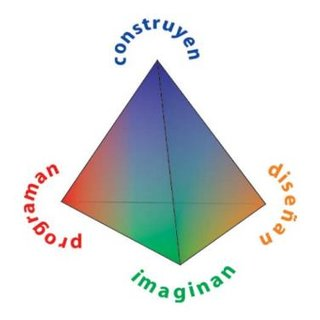
\includegraphics[width=0.3\textwidth]{images/metodologia.png}
  \caption{Las cuatro palabras de la Robótica educativa (Báez \textit{et al}., 2011).}
  \label{Metodologia}
\end{figure}
\\
En la última década, la robótica ha adquirido mucha importancia en un gran número de países (Quiroga, 2018), y cada vez genera mas interés implantarla en las aulas (Salamanca, Barrera y Pérez, 2010). Esto se debe a que aporta muchos beneficios en el proceso de enseñanza-aprendizaje de asignaturas difíciles (Moreno \textit{et al}., 2012) y permite alcanzar un mejor desarrollo en materias de ciencias, tecnología o matemáticas. Por ello, la robótica puede considerarse una enseñanza STEM (acrónimo de \textit{Science, Technology, Engineering and Mathematics}) (Figura 1.6), un término acuñado en lo años 90 por la NSF (\textit{National Science Foundation}) que sirve para designar aquellos ámbitos que permiten formase en esas cuatro áreas de conocimiento.
\\
\begin{figure}[h!]
  \centering
    \includegraphics[width=0.5\textwidth]{images/educacion_stem.png}
  \caption{Enseñanza STEM}
  \label{Enseñanza STEM}
\end{figure}
\\
Otro aspecto importante es que, debido a las crecientes aplicaciones robotizadas en las empresas, se necesita incluir más profesionales formados en este sector. Por ello, si se empieza a enseñar desde edades tempranas se obtendrá una mejor formación en este ámbito (Hernández, 2019). Esta era una de las intenciones del Decreto 89/2014 del 24 de julio, que añade en el currículo de la Educación Primaria de la Comunidad de Madrid la asignatura “Tecnología y recursos digitales para la mejora del aprendizaje”, cuyos contenidos incluyen los fundamentos de la programación y la programación de juegos sencillos. Además, el Decreto 48/2015 del 14 de mayo, también añadió la asignatura “Tecnología, Programación y Robótica” en el currículo de la Educación Secundaria de la Comunidad de Madrid, con materias sobre la programación y el pensamiento computacional, la robótica y su relación con el mundo real, diseño e impresión 3D,  Internet y su uso responsable y desarrollo del aprendizaje basado en proyectos (Instituto Nacional de Tecnologías Educativas y de Formación del Profesorado, 2018).
\\
\\
También ha sido de gran ayuda la creación de lenguajes de programación orientados a alumnos de menor edad, así como la aparición de empresas orientadas a distribuir kits de robótica para STEM. En el primer caso, destaca el lenguaje \texttt{Scratch} (Figura 1.7), diseñado por el MIT (\textit{Massachusetts Institute of Technology}) y que consiste en un lenguaje de programación visual y basado en bloques que permite desarrollar la creatividad y el pensamiento lógico de una manera sencilla (Penalva, 2019).
\\
\begin{figure}[h!]
  \centering
    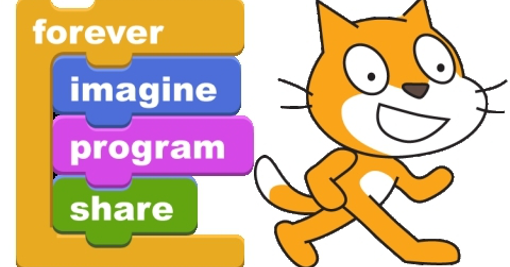
\includegraphics[width=0.3\textwidth]{images/logo_scratch.png}
  \caption{Lenguaje de programación Scratch}
  \label{Lenguaje de programación Scratch}
\end{figure}
\\
Respecto a los kits de robótica existentes en el mercado, algunos de los más populares son (Figura 1.8):
\begin{itemize}
	\item \textbf{Mbot.} Diseñado por la empresa MackeBlock y basado en Arduino Uno.

	\item \textbf{Mindstorms Education EV3.} Fabricado por LEGO. Permite diseñar diferentes robots gracias a las piezas de LEGO. Dispone de una pequeña computadora programable llamada EV3.
			
	\item \textbf{VEX Robotics.} Se trata de un proveedor de productos de robótica educativa que diseña kits para estudiantes de diferentes edades. Sus kits están basados en piezas, con las que el alumno podrá diseñar un gran número de robots. Incluye tres tipos de kits: el \textit{VEX IQ}, orientado para estudiantes de primaria y secundaria al tener piezas de plástico y no necesitar herramientas para su montaje, el \textit{VEX EDR}, orientado para alumnos más mayores y que utiliza piezas metálicas para la construcción de los robots y el \textit{VEX PRO}, orientado a profesionales de la robótica.
	
	\item \textbf{Root Robot.} Diseñado por iRobot Educational. Su objetivo es mejorar la enseñanza en temas relacionados con la codificación, creatividad y resolución de problemas.
\end{itemize}
\begin{figure}[h!]
  \centering
    \includegraphics[width=0.7\textwidth]{images/kits_robotica.png}
  \caption{Mbot (esquina superior izquierda), Mindstorms EV3 (esquina superior derecha), ejemplo de robot construido con VEX (esquina inferior izquierda) y Root Robot (equina inferior derecha)}
  \label{Mbot, Mindstorms EV3, ejemplo de robot construido con VEX  y Root Robot}
\end{figure}

Existen aplicaciones y entornos web de programación robótica que facilitan la creación de programas para los robots, como pueden ser MBlock (desarrollada por la empresa MakeBlock y basada en Scratch 3), Bitbloq (creada por la empresa BQ, que utiliza bloques para realizar los programas y es compatible con la placa \texttt{Arduino}), Open Roberta Lab (entorno de programación web diseñado por Google, que permite programar algunos de los robots más famosos como el EV3 y también robots simulados) o Kibotics.
\\
\\
Por último, se han creado competiciones que permiten que los alumnos se diviertan diseñando y programando sus robots. Algunas de ellas son:
\begin{itemize}
	\item \textit{First LEGO League:} realizada desde el 2006 por la Fundación Scientia. Reúne a centros escolares y los alumnos deben solucionar un problema planteado que cambian en cada edición.

	\item \textit{RoboCup Junior:} una de las más famosas. Sus tres modalidades se basan en un 2 contra 2 de fútbol robótico, robots de rescate y diseño de una coreografía de robots bailarines.
		
	\item \textit{Robocampeones:} dedicada para alumnos de secundaria y bachillerato. Entre sus modalidades destaca la competición de sumo robótico.
	
\end{itemize}



\section{Kibotics}

Kibotics\footnote{\url{https://kibotics.org/}}, es un entorno web desarrollado por la Asociación JdeRobot\footnote{\url{https://jderobot.github.io/}} para la docencia de robótica, programación y áreas STEM. Fue ideada para ayudar a los alumnos a iniciarse en el mundo de la robótica y la programación de forma
sencilla y práctica.
\\
\\
Es una plataforma con un gran potencial debido a sus características. Es multirobot, dentro de ella podemos encontrar distintos ejercicios tanto de robots simulados (p. ej. un Fórmula Uno) como de robots reales (p. ej. Pibot, figura 1.9). Posee una evaluación automática sobre los ejercicios y correcciones de estilo. También incluye ejercicios orientados a la visión artificial utilizando las cámaras de los robots.
\\
\begin{figure}[h!]
  \centering
    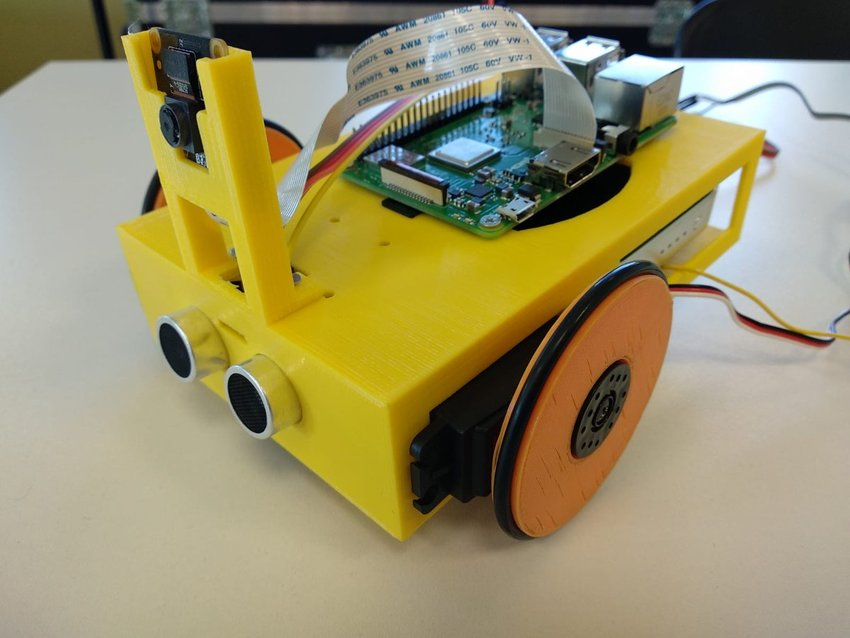
\includegraphics[width=0.4\textwidth]{images/pibot.png}
  \caption{Robot PiBot}
  \label{Robot PiBot}
\end{figure}
\\
En cuanto a los lenguajes reconocidos por esta plataforma, encontramos \texttt{Blockly} y \texttt{Python}. El primero de ellos fue desarrollado por Google y es muy similar a \texttt{Scratch}. Está orientado para alumnos de menor edad por ser un lenguaje de programación visual basado en una interfaz de bloques que se pueden encajar como si fuera un puzle. Su uso en colegios e institutos es cada vez mayor, ya que esta diseñado para que la iniciación al mundo de la programación sea sencilla, divertida y creativa (Figura 1.10).
\\
\begin{figure}[h!]
  \centering
    \includegraphics[width=1\textwidth]{images/kibotics_blockly.png}
  \caption{Ejercicio con Blockly en Kibotics}
  \label{Ejercicio con Blockly en Kibotics}
\end{figure}
\\
\texttt{Python}, por su parte, está enfocado para alumnos mayores. Constituye uno de los lenguajes de programación con más popularidad en la actualidad según el Índice de Popularidad de Lenguajes de Programación\footnote{\url{http://pypl.github.io/PYPL.html}}. Gracias a la sencillez de su sintaxis, es muy utilizado para iniciarse en la programación.
\\
\begin{figure}[h!]
  \centering
    \includegraphics[width=1\textwidth]{images/kibotics_python.png}
  \caption{Ejercicio con Python en Kibotics}
  \label{Ejercicio con Python en Kibotics}
\end{figure}
\\


%###############################################################################
%############# OBJETIVOS #######################################################
%###############################################################################


\chapter{Objetivos}

Una vez presentado el marco en el que se realiza este trabajo, en este capítulo se exponen los objetivos propuestos y los requisitos de este proyecto, además de la metodología de trabajo que se ha llevado a cabo para su resolución.

\section{Objetivos del TFG}

El objetivo principal de este trabajo es conseguir integrar nuevos robots reales en la plataforma Kibotics para poder programarlos desde ella.
\\
\\
En concreto, en este proyecto se pretende dar soporte a tres robots diferentes. Cada uno de estos robots presenta una serie de características propias que le hace ser interesante y distinto, motivo por el cual supone un gran enriquecimiento para esta plataforma.
\begin{itemize}
	\item \textit{Mbot.} Se ha elegido por ser uno de los más populares en el mundo de la Robótica Educativa, ya que tiene un diseño muy atractivo para los niños. Además, está basado en la placa \texttt{ArduinoUno}, una de las placas más famosas de código abierto y de la que hay mucha documentación y ejemplos de ejercicios que ayudan en el aprendizaje.
	\item \textit{Tello.} Este dron ofrece muy buenas cualidades para aprender, fácil y económicamente, a programar este tipo de robots, los cuales han adquirido una gran popularidad en los últimos años, tanto a nivel profesional como para el entretenimiento.
	\item \textit{GoPiGo3.} Este robot, cuya placa controladora es una Raspberry Pi, se ha convertido en un robot muy inteligente y versátil. Soporta visión; se le puede conectar una cámara vía USB o mediante un puerto dedicado especialmente a la \textit{Pi Camera}. Esto le otorga una amplia gama de posibilidades para realizar programas relacionados con la visión artificial: detección de objetos, análisis de imagen, etc.
\end{itemize}
Gracias a estos robots, los alumnos no solo aprenden temas relacionados con la robótica, sino que también van a introducirse en el mundo de la informática y la electrónica.
\\
\\
Hasta el momento, Kibotics incluye algunos robots reales para poder programarlos, entre ellos el ya mencionado Mbot. Sin embargo, este robot solo puede programarse utilizando un ordenador con Linux como sistema operativo. Además, el proceso de enviarle el programa no es directo, pues cuando el usuario quiere enviar el programa realizado al robot, es necesario descargar un ejecutable.

\section{Requisitos}

La integración en Kibotics de los citados robots se realizará, además, siguiendo los siguientes objetivos específicos.
\begin{itemize}
	\item \textit{Multiplataforma.} La programación de estos robots será soportada por los principales sistemas operativos (Linux, Windows y MacOS).
	\item \textit{Sin instalación.} El proceso de envío del programa al robot debe ser lo más sencillo posible para evitar que el usuario tenga que hacer instalaciones o configuraciones adicionales. De esta manera conseguimos que las personas con pocos conocimientos en informática también puedan hacer uso de la plataforma.
\end{itemize}
Con todo lo anterior, se pretende dar continuidad al objetivo principal de Kibotics: acercar la robótica al público más general y a los más pequeños.

\section{Metodología}

Para el desarrollo de este trabajo se ha seguido el modelo de diseño iterativo (Figura 2.1), muy utilizado en el desarrollo de software. Se basa en la idea de entregar al cliente algo tangible cuanto antes para que pueda validarlo y, si es necesario, puedan hacerse los cambios de manera rápida sin tener que modificar todo el proyecto por completo. Además, también se deben hacer pequeñas iteraciones para evaluar las funcionalidades en los siguientes ciclos. Este diseño es una buena opción porque aporta cierta flexibilidad, algo muy útil en los procesos de desarrollo del software, los cuales suelen experimentar cambios frecuentes.
\\
\begin{figure}[h!]
  \centering
    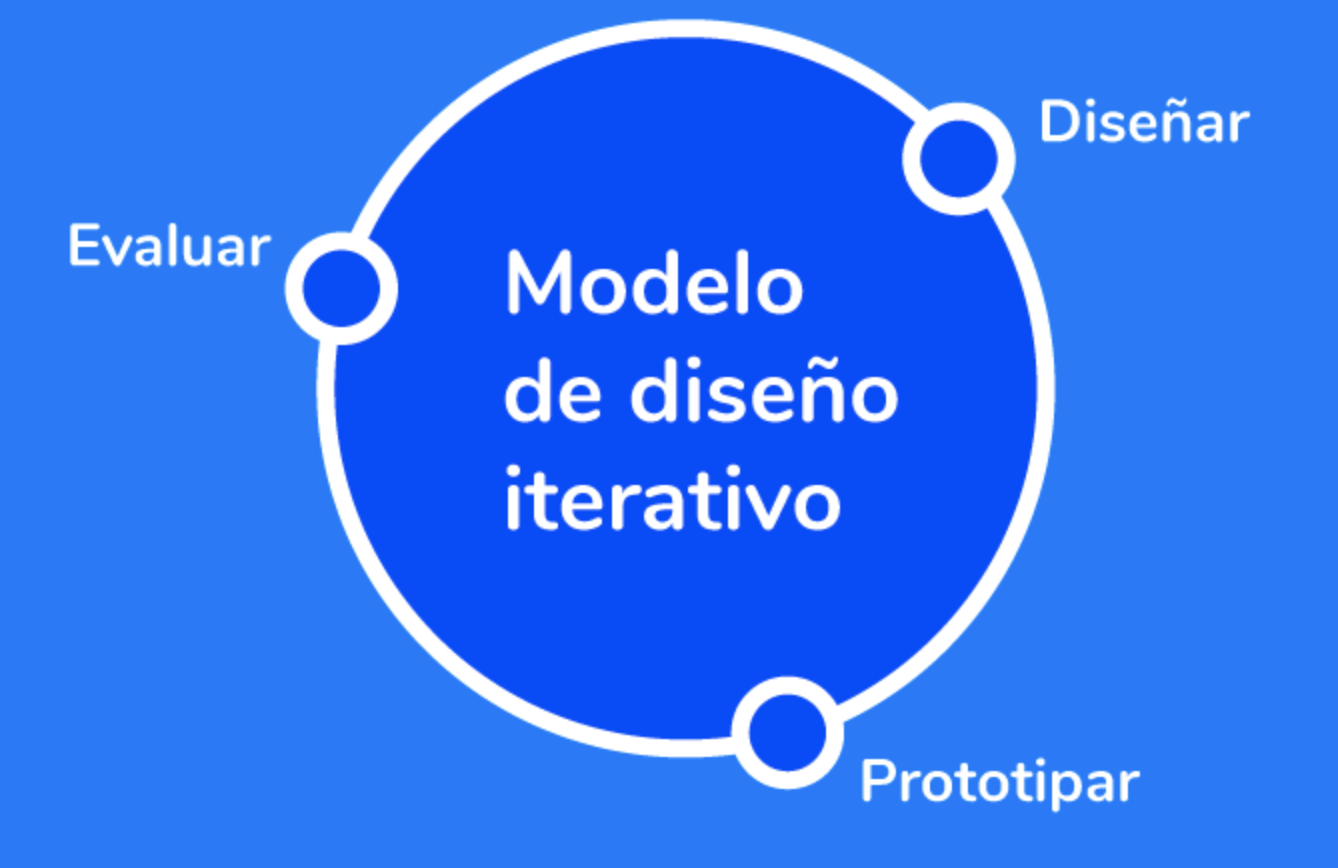
\includegraphics[width=0.5\textwidth]{images/metodologia_interativa.png}
  \caption{Modelo iterativo}
  \label{Modelo iterativo}
\end{figure}
\\
La ventaja de usar esta metodología es que los tutores no tienen que esperar mucho tiempo hasta ver resultados del proyecto, por lo que pueden revisar e ir dando sus opiniones y realimentaciones de forma rápida. De este modo, al hacer varias iteraciones, el riesgo ante un problema es pequeño y fácil de solucionar. Todo esto hace que el conocimiento sobre el producto sea progresivo y creciente.
\\
\\
Así, para el seguimiento de este trabajo, se ha utilizado la herramienta de control de versión \texttt{Git} y \texttt{GitHub}. Además, se planificaban reuniones semanales con los tutores del TFG y se creó un blog \footnote{\url{https://roboticslaburjc.github.io/2019 tfg-david-valladares/}} donde se registraban las tareas realizadas a lo largo de la semana (Figura 2.2).
\\
\begin{figure}[h!]
  \centering
    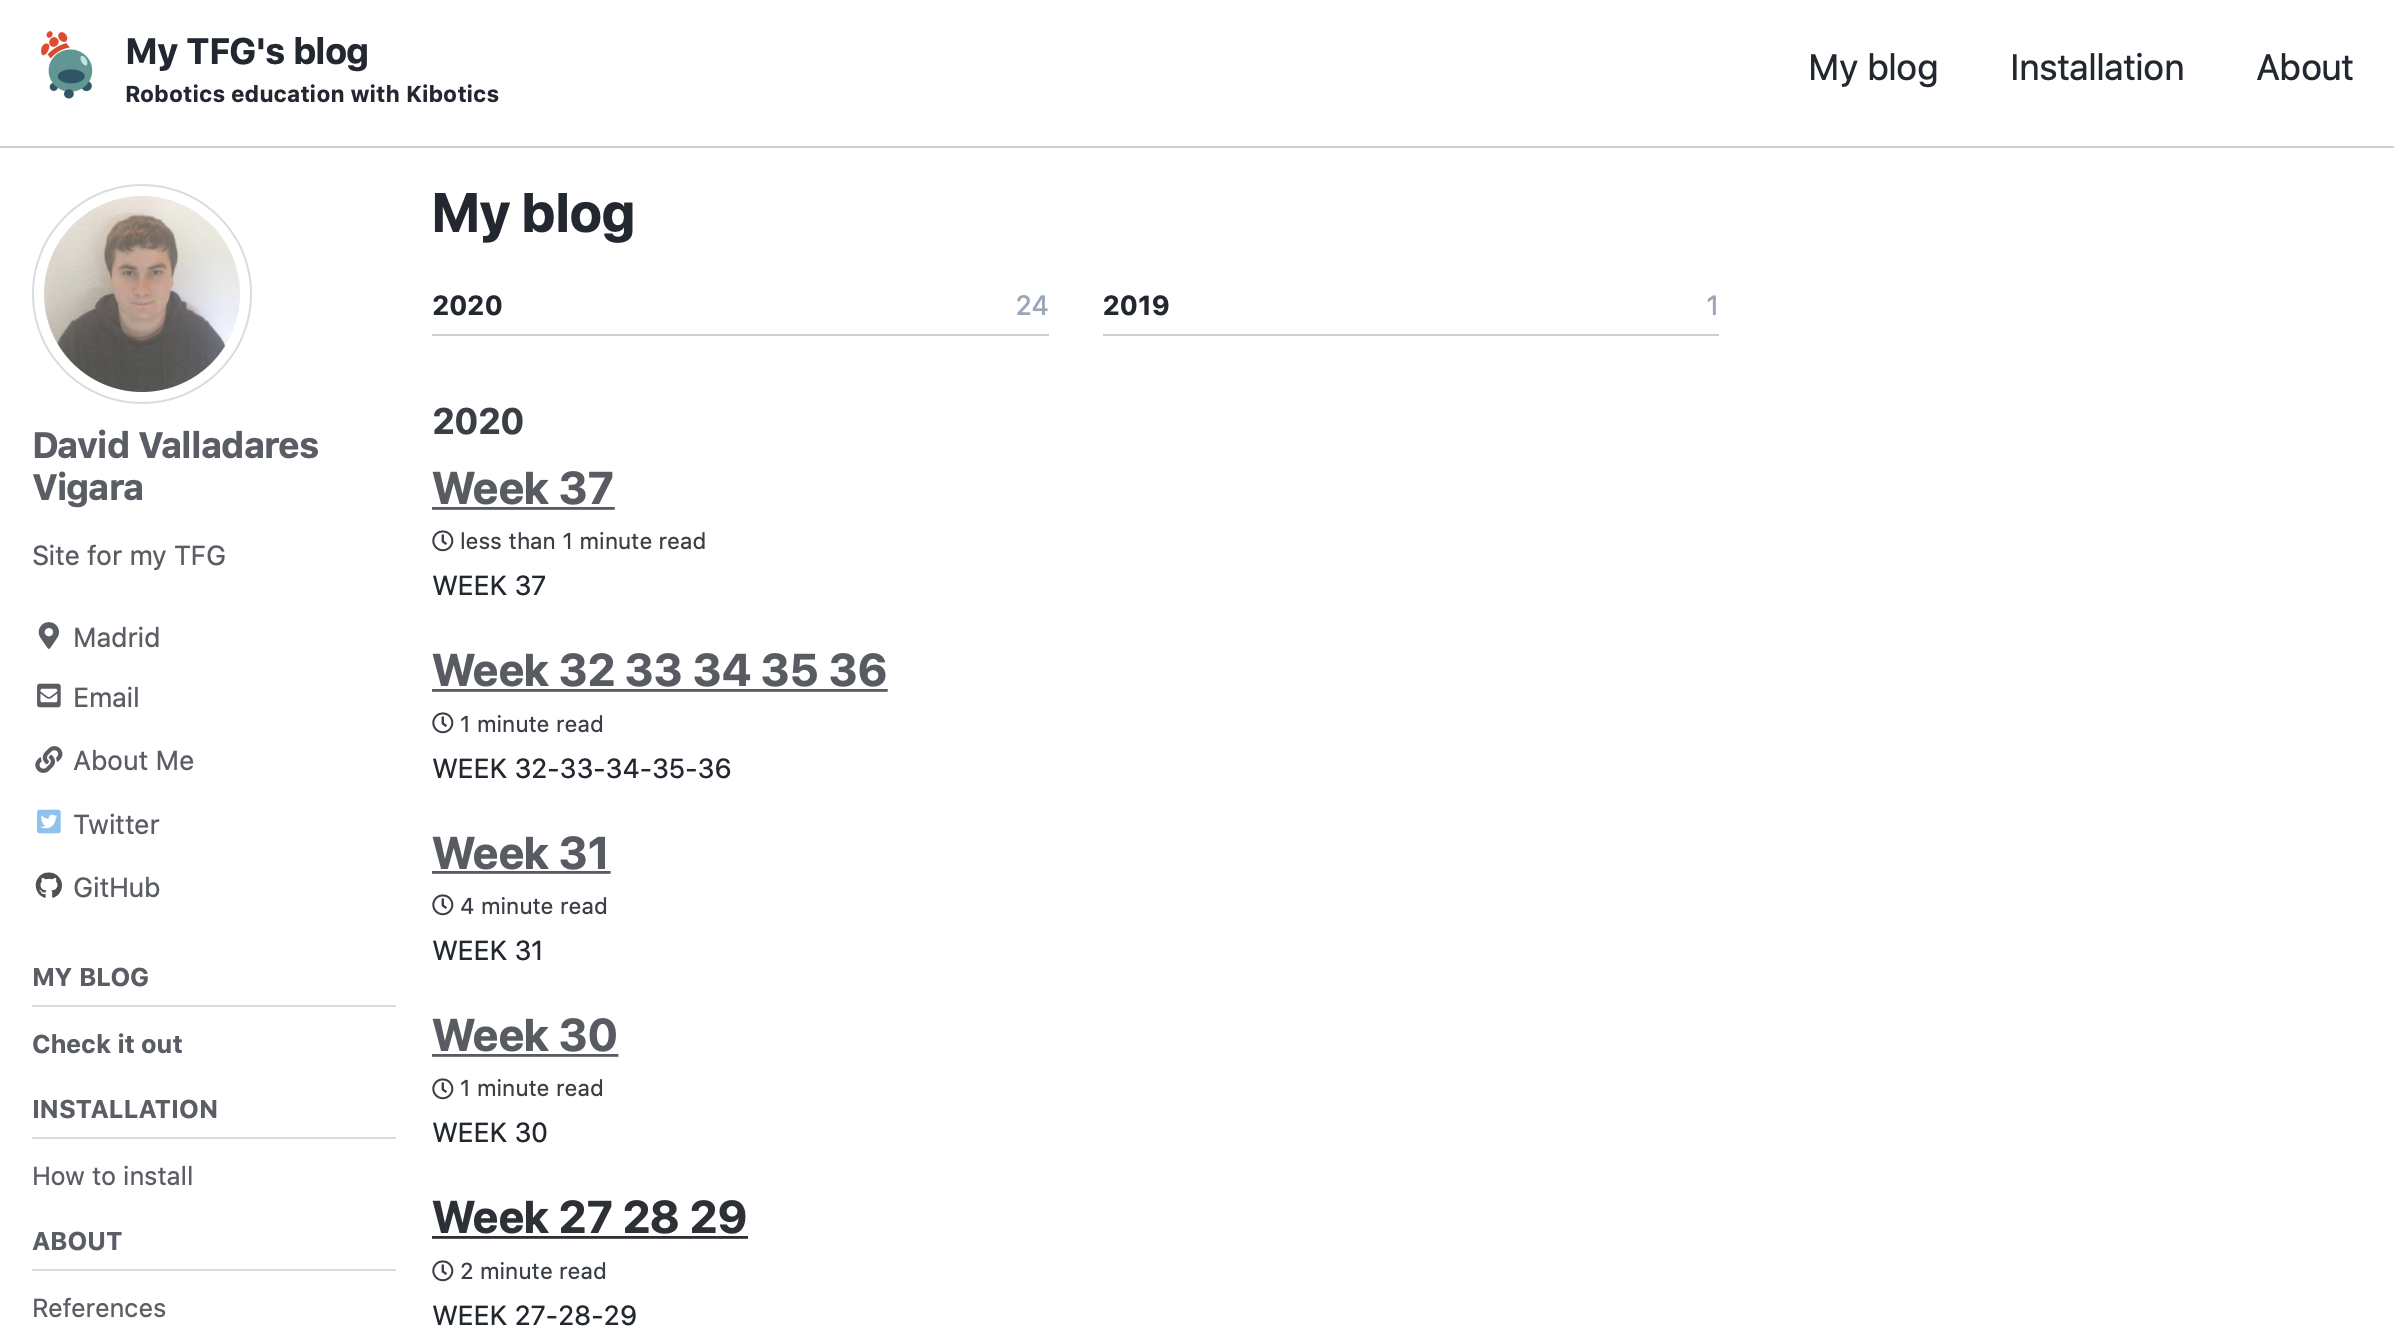
\includegraphics[width=1\textwidth]{images/blog.png}
  \caption{Blog para el seguimiento del TFG}
  \label{Blog para el seguimiento del TFG}
\end{figure}

\section{Plan de trabajo}

El plan de trabajo que se ha seguido durante la elaboración del proyecto puede dividirse en las siguientes etapas:
\begin{itemize}
	\item \textit{\textbf{Aterrizaje en la plataforma de Kibotics.}} Esta plataforma web está montada sobre un servidor usando la tecnología \texttt{Django}, por lo que se tuvo que aterrizar en cómo consistía el funcionamiento de esta aplicación.
	\item \textit{\textbf{Diseño para el Mbot.}} En el inicio de esta fase fue fundamental entender el API de \texttt{Web Serial} y de las características del propio robot. Se hizo un primer prototipo de ejemplo para ver la interacción con una placa \texttt{ArduinoUno}. Posteriormente, se realizó la integración en la plataforma y se perfiló la interfaz y la usabilidad del envío del programa al robot.
	\item \textit{\textbf{Diseño para el dron Tello.}} Al igual que en la fase anterior, también se empezó estudiando las características del robot y del uso de \texttt{PyInstaller}. La primera integración que se diseñó fue para los ordenadores con \texttt{Linux} y, después, se procedió con el diseño de la integración para \texttt{MacOS} y \texttt{Windows}.
	\item \textit{\textbf{Diseño para el GopiGo3.}} En este caso, además de conocer las características del robot, también fue necesario aprender a manejar la Raspberry Pi y entender la librería \texttt{Flask}. Se desarrolló un primer prototipo de ejemplo para encender un led en la placa \texttt{Arduino} vía web. Después, se realizó la integración en Kibotics y se mejoró la interfaz y usabilidad del envío del programa.
	
\end{itemize}





%###############################################################################
%############# HERRAMIENTAS ###################################################
%###############################################################################

\chapter{Herramientas}

En este capítulo se describen las herramientas que han sido utilizas para el desarrollo de este trabajo de fin de grado.

\section{Lenguaje Python}

Python es un lenguaje de programación diseñado por Guido Van Rossum y publicado en el año 1991 (Challenger, Díaz y Becerra, 2014). Es un proyecto de código abierto gestionado por Python Software Foundation, una sociedad sin ánimo de lucro. Actualmente se encuentra en su versión 3.8 (Zaforas, 2018).
\\
\\
Presenta algunas características que implican una serie de ventajas para los usuarios y que son las responsables de su gran popularidad. En primer lugar, se trata de un lenguaje multiparadigma, es decir, permite utilizar diferentes paradigmas de programación, como son la orientación a objetos, funcional o imperativa. Además, al ser un lenguaje interpretado, no necesita ser compilado ni enlazado. Posee un tipado dinámico (aunque desde la versión 3.5 puede hacerse uso del tipado estático), y es multiplataforma, lo que significa que puede ser ejecutado en diferentes sistemas operativos (Zaforas, 2018). La sintaxis de Python es más sencilla que la de otros lenguajes de programación, algo muy importante para la educación. Además, cuenta con una de las librerías más completas, comparable a la de Java y .NET (Challenger, Díaz y Becerra, 2014). Todo esto le han convertido en uno de los lenguajes de programación más utilizados en la actualidad.

\section{Lenguaje HTML}

HTML (HyperText Markup Languaje) fue desarrollado en 1991 por Tim Berners-Lee mientras trabajaba en la Organización Europea para la Investigación Nuclear (CERN), y popularizado por el navegador Mosaic desarrollado en NCSA (Raggett, Le Hors y Jacobs, 1999).
\\
\\
No es un lenguaje de programación, es decir, no tiene capacidad de crear una funcionalidad dinámica, sino que consiste en un lenguaje de marcado de hipertexto, basado en el metalenguaje SGML (Standard Generalized Markup Language). Este lenguaje da formato a los documentos de la WWW (World Wide Web) (Lamarca, 2018). Se podría considerar un lenguaje entendido universalmente por todos los ordenadores que permite que la información publicada tenga una distribución global (Raggett, Le Hors y Jacobs, 1999).
\\
\\
La organización W3C (World Wide Web Consortium) es quien lleva a cabo las especificaciones relativas a este lenguaje. Está definido por “etiquetas” que el navegador interpreta y da forma en la pantalla. Estas etiquetas encierran un contenido y, todo en conjunto, forman lo que se denomina “elemento” (Lamarca, 2018).
\\
\begin{lstlisting}[frame=single,breaklines=true, label=Ejemplo de código HTML, caption=Ejemplo de código HTML, captionpos=b]
<!DOCTYPE html>
<html>
  <head>
    <meta charset="utf-8">
    <title>Mi pagina de prueba</title>
  </head>
  <body>
    <img src="images/firefox-icon.png" alt="Mi imagen de prueba">
  </body>
</html>

\end{lstlisting}

\section{Lenguaje JavaScript}

JavaScript es un lenguaje de programación desarrollado por Brendan Eich a finales de los años 90. Se considera un lenguaje interpretado, de tipado débil y dinámico, y se utiliza, principalmente, para crear páginas web dinámicas en el lado del cliente, es decir, aquellas que incluyen efectos, animaciones, ventanas emergentes… (Eguíluz, 2009). Sin embargo, actualmente también existe la posibilidad de ejecutar JavaScript en todo tipo de desarrollo de aplicaciones (NodeJs).
\\
\\
Su nombre se debe a que los programas o aplicaciones creados con este lenguaje de programación se denominan “script” (Eguíluz, 2009). Además, su sintaxis es muy similar a la de otros lenguajes (Java y C)

\section{Bootstrap}

Bootstrap (Figura 3.1) fue diseñado por Mark Otto y Jacob Thornton para crear mejores herramientas internas en Twitter, aunque en agosto de 2011 pasó a ser de código abierto, lo que favoreció su desarrollo (Cumplido, 2018).
\\
\\
Consiste en un framework utilizado para el desarrollo web basado en CSS (Cascading Style Sheets), un lenguaje que permite estructurar y componer páginas web, y JQuery, una librería de JavaScript utilizada para dotar de interactividad a una web. Utiliza un sistema de rejillas (cuadrículas) para el diseño de la web. Este framework facilita la tarea de maquetar una página web, creando así una interfaz muy limpia y adaptable al tamaño de la pantalla del dispositivo. Es compatible con los principales navegadores (Firefox, Google Chrome, Safari), lo que supone una gran ventaja. Además, existe una gran cantidad de documentación disponible, lo que facilita su uso y comprensión (Guevara, s.f.).
\\
\begin{figure}[h!]
  \centering
    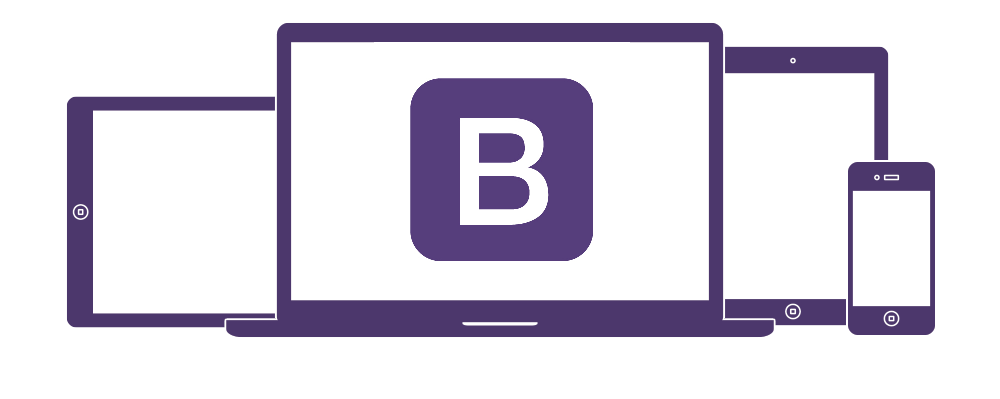
\includegraphics[width=0.5\textwidth]{images/bootstrap.png}
  \caption{Bootstrap}
  \label{Bootstrap}
\end{figure}

\section{Django}

Django es un framework de código abierto escrito en Python, creado en 2005, el cual permite desarrollar un entorno web complejo de una forma rápida y estructurada. Actualmente es mantenido por Django Software Foundation y se encuentra en la versión 3.0 (Novapros, 2020).
\\
\\
Sigue una arquitectura MVC (Modelo – Vista - Controlador), como se observa en la figura 3.2 (Holovaty y Kaplan-Moss, 2007).
\begin{itemize}
	\item \textit{Modelo}. Los modelos de datos creados están mapeados directamente a las tablas de la base de datos, permitiendo aislar el código de la aplicación de la base de datos.

	\item \textit{Vista}. Corresponde con la capa de presentación, y está basada en plantillas HTML.		
	\item \textit{Controlador (en Django llamado “views”)}. Responsable de seleccionar la plantilla a mostrar. Atiende a una petición y, según el mapeo de la URL, (Uniform Resource Locator) redirige a una vista u otra.
\end{itemize}
Ofrece una serie de características bastante interesantes como es su excelente capa de seguridad (p ej. permite una protección contra los ataques maliciosos “Cross-site request forgery”), dispone de un sistema de administrador “por defecto,” sin necesidad de realizar ningún tipo de configuración. También proporciona una interfaz para el acceso a la base de datos, facilitando las consultas (Novapros, 2020).
\begin{figure}[h!]
  \centering
    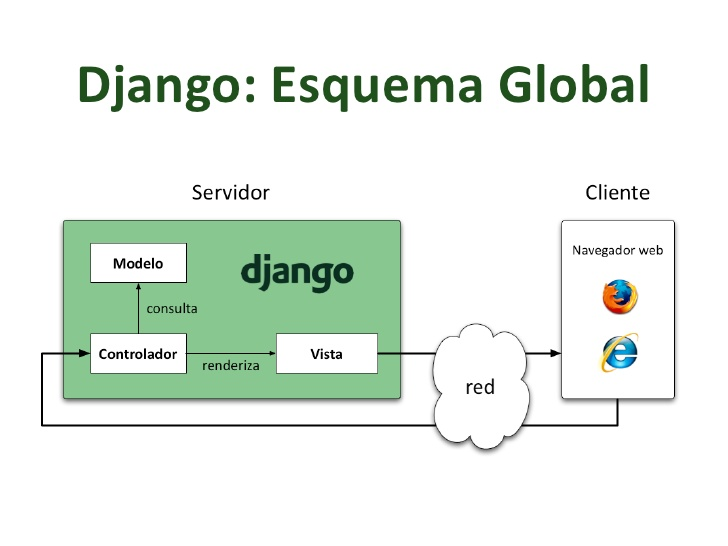
\includegraphics[width=0.6\textwidth]{images/django.png}
  \caption{Arquitectura Django}
  \label{Arquitectura Django}
\end{figure}

\section{Flask}

Flask (Figura 3.3), lanzado en abril de 2010 es, junto con Django, uno de los framework webs más famosos escritos en Python.
\\
\\
Está enfocado en proporcionar lo mínimo necesario para poner en funcionamiento una aplicación, por eso se le considera un framework “minimalista”. Por otro lado, no requiere de otras dependencias para realizar acciones básicas, de manera que la curva de aprendizaje para su comprensión es muy baja. Debido a su sencillez en la estructura, posee una velocidad mayor que Django y es bastante útil para iniciarse en el aprendizaje de desarrollo web, permitiendo crear servidores de una forma rápida. Debido a ello, Flask está orientado al sector servicios, los cuales implican muchas visitas y una carga grande de peticiones, y también para proyectos personalizados o sencillos (Rodríguez, 2019).
\begin{figure}[h!]
  \centering
    
\includegraphics[width=0.4\textwidth]{images/flask.png}
  \caption{Arquitectura Django}
  \label{Arquitectura Django}
\end{figure}

\section{Web Serial Api}

Web Serial es una Api (Application Programming Interface) JavaScript, especificada por WICG (Web Platform Incubator Community Group), que permite interactuar con dispositivos conectados al puerto serie del ordenador desde un navegador web. Actualmente esta Api es soportada por los navegadores de escritorio basados en Chromium (Google Chrome, Opera, Edge), pero para poder utilizarla es necesario habilitarla.
\\
\\
Muchos dispositivos periféricos que se conectan al ordenador requieren de una descarga software para controlarlo. Un claro ejemplo de esto se ve en la robótica; en la mayoría de los robots en los que la carga del programa se realiza por USB (Universal Serial Bus), es necesario instalar previamente en el ordenador un software que permita hacerlo. La ventaja de Web Serial es que  proporciona una vía capaz de comunicarse con estos dispositivos sin necesidad de instalar nada en el ordenador (W3C Community Group, 2020).

\section{PyInstaller}

PyInstaller es un módulo lanzado por la línea de comandos que permite agrupar aplicaciones Python en un único paquete junto con todas las dependencias necesarias y el intérprete de Python, permitiendo crear un ejecutable para ser distribuido. Es compatible con las versiones de Python 2.7 y para las versiones superiores a Python3.3. Puede ser utilizado para Linux, Windows y MacOS, aunque no permite una compilación cruzada, es decir, la aplicación empaquetada solo puede utilizarse en el mismo sistema operativo en el que fue empaquetado, por lo que una aplicación empaquetada en Linux no podrá ser utiliza en una computadora con Windows o MacOS (SO Documentation, s.f.).
\\
\begin{lstlisting}[frame=single,breaklines=true, label=Ejemplo para generar un ejecutable con PyInstaller, caption=Ejemplo para generar un ejecutable con PyInstaller, captionpos=b]
 		   $ pyinstaller -onefile hello.py
\end{lstlisting}

\section{Placa mCore}

La placa mCore (Figura 3.4) está basada en una placa ArduinoUno, una microcontroladora de código abierto que utiliza un microchip ATmega328P, pero extendida con más componentes y que, además, incorpora la electrónica de potencia para el manejo de los motores.
\\
\begin{figure}[h!]
  \centering
    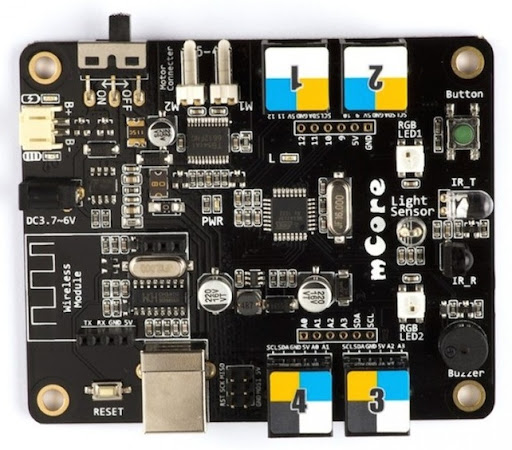
\includegraphics[width=0.5\textwidth]{images/mcore.png}
  \caption{Placa mCore}
  \label{Placa mCore}
\end{figure}
\\
La placa permite ser programada a través del puerto serie gracias al bootloader, un software alojado en la memoria flash. En el arranque de la placa, el bootloader comprueba si se está intentado programarla y, en caso afirmativo, se procede a grabar el programa en la memoria y se reinicia. En el caso contrario, el bootloader ejecuta el último programa que estuviera grabado. Estas placas pueden ser programadas utilizando el lenguaje Arduino, un lenguaje de alto nivel que está basado en el lenguaje C++, pero adaptado para facilitar la programación de los pines de entrada y salida (Llamas, 2016).
\\
\\
Una vez que el programa ha sido escrito en este lenguaje de alto nivel, es necesario compilarlo para obtener el código ejecutable entendido por la placa para el proceso de carga (Figura 3.5).
\\
\begin{figure}[h!]
  \centering
    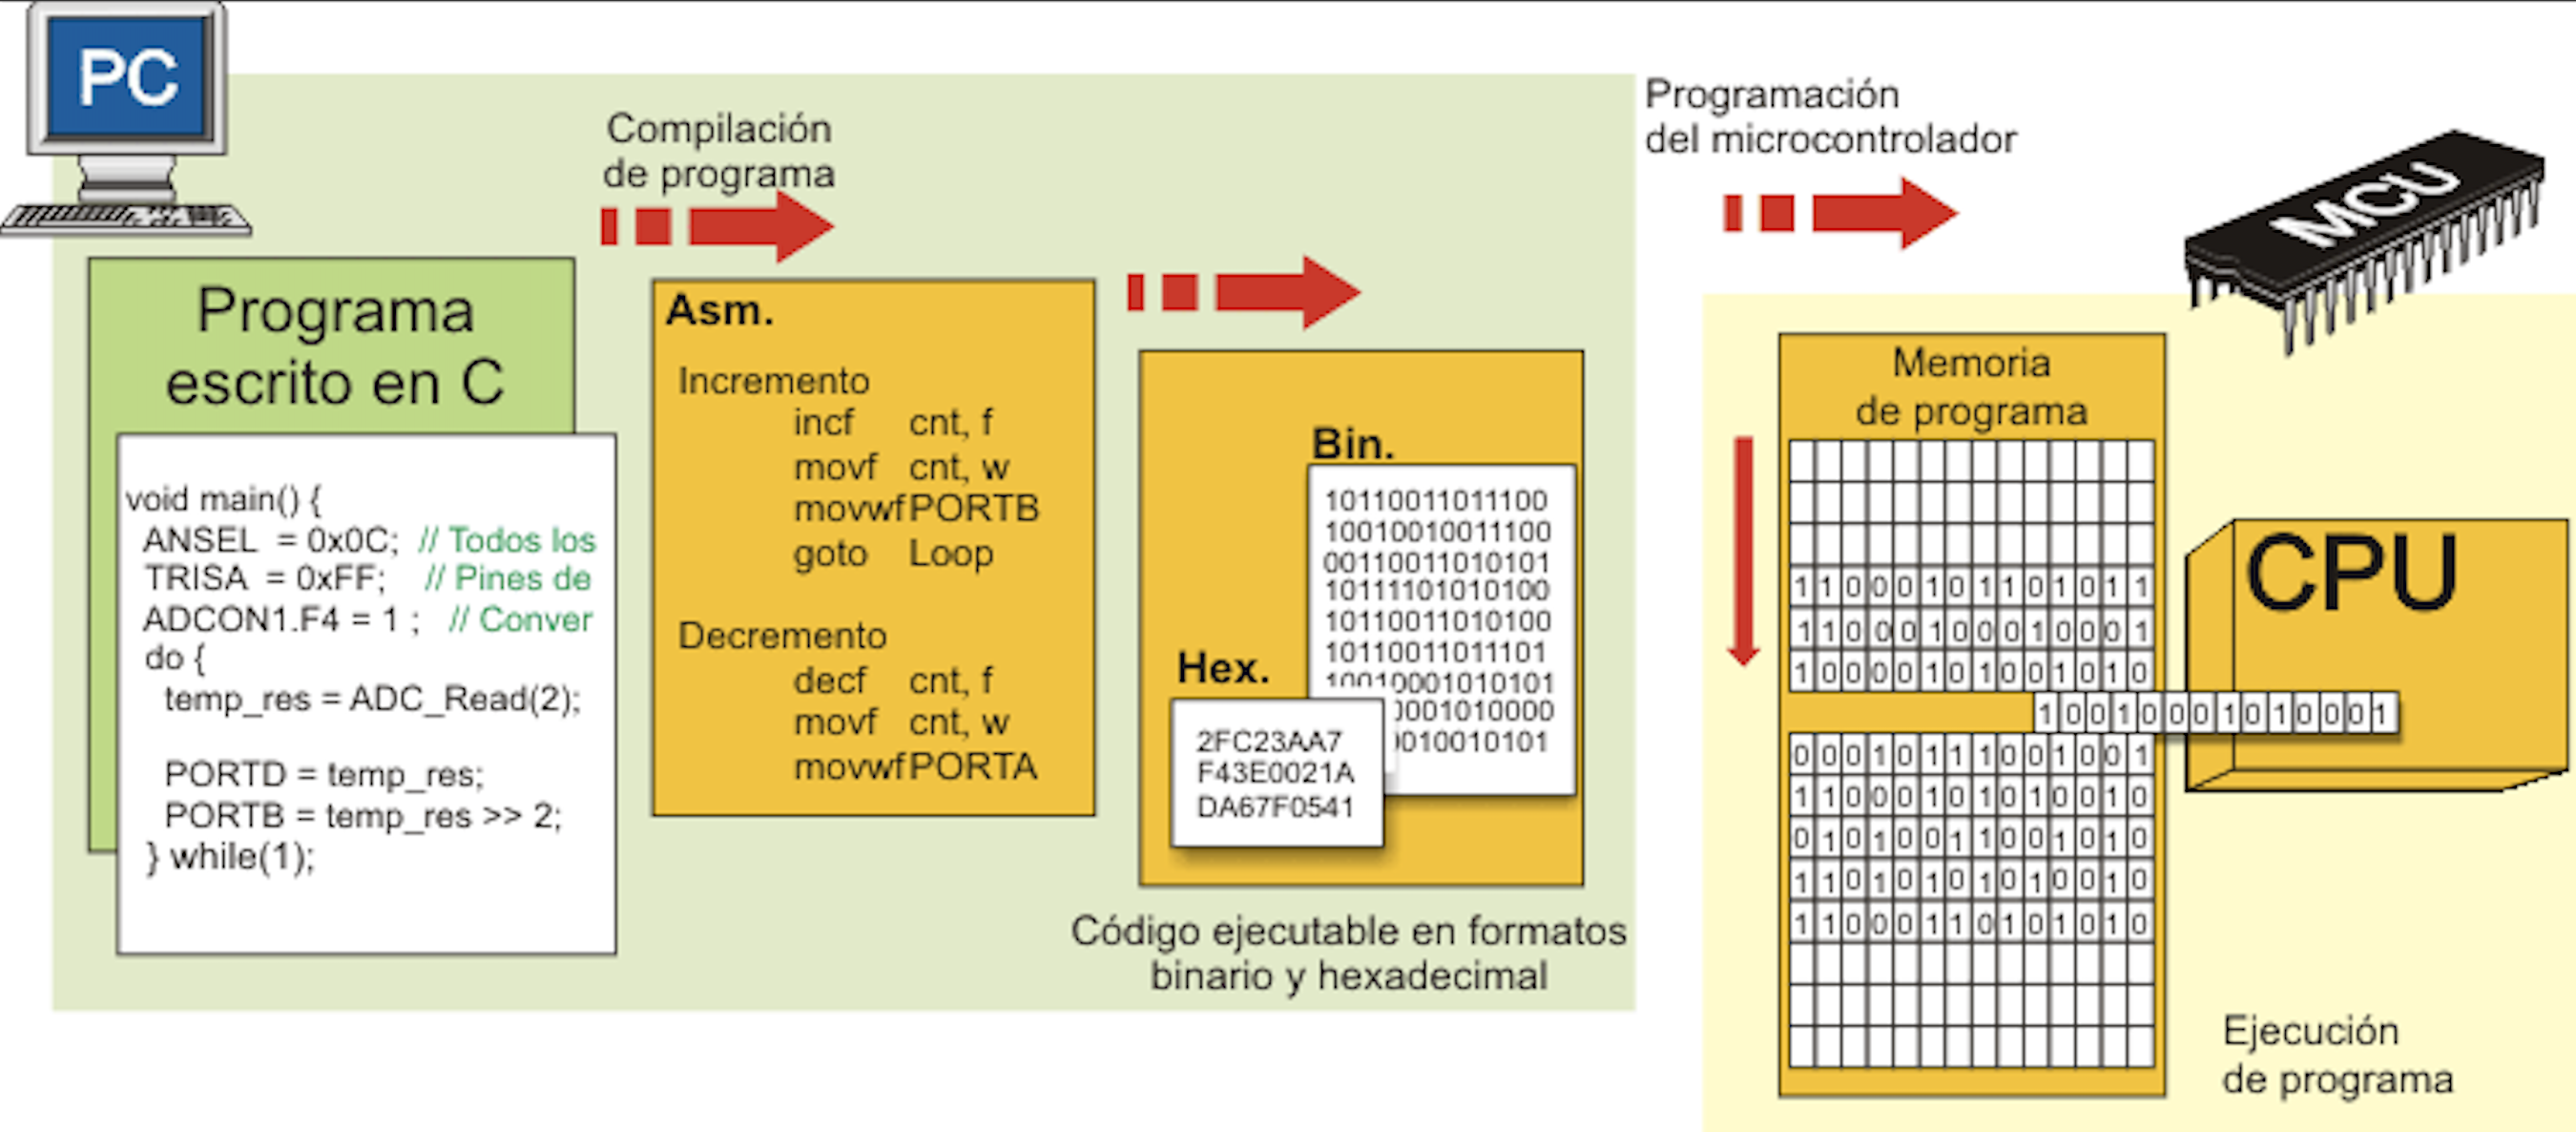
\includegraphics[width=1\textwidth]{images/carga_mcore.png}
  \caption{Proceso de carga de un programa a la placa mCore}
  \label{Proceso de carga de un programa a la placa mCore}
\end{figure}

\section{Raspberry Pi}

Raspberry Pi es un proyecto que nace en 2009 en Londres bajo la asociación caritativa denominada Fundación Raspberry Pi, cuyo objetivo era mejorar la enseñanza de la informática en las aulas.
\\
\\
Consiste una placa computadora de bajo coste que puede considerarse como un ordenador de tamaño reducido. Su hardware se compone, principalmente, de una CPU (Central Processing Unit), una GPU (Graphics Processing Unit), una memoria RAM (Random Access Memory), una ranura SD (Secure Digital) utilizada para el almacenamiento, salidas y entradas de audio y vídeo, pines de entrada y salida de propósito general (GPIO), bus USB, tarjeta de red y alimentación. En cuanto a su software, existen una gran cantidad de sistemas operativos que pueden usarse, tales como  Raspbian, Kali Linux, Windows 10 IoT Core, Ubuntu Core… (Escuela Técnica Superior de Ingeniería Informática de la Universidad Politécnica de Valencia, 2013).
\\
\\
Este ordenador es muy utilizado en la actualidad gracias a la gran variedad de usos que puede ofrecer, ya que puede emplearse como un ordenador de sobremesa, utilizarse en Robótica, como un dispositivo para la domótica…
\\
\\
Para este TFG, hemos usado la Raspberry Pi 3 modelo B. En la figura 3.6 se muestran sus características principales.
\\
\begin{figure}[h!]
  \centering
    \includegraphics[width=1\textwidth]{images/hardware_RaspberryPi.png}
  \caption{Características hardware para la Raspberry Pi modelo 3B}
  \label{Características hardware para la Raspberry Pi modelo 3B}
\end{figure}














%###############################################################################
%###################### MBOT ###################################################
%###############################################################################

\chapter{Integración del robot Mbot}

En este capítulo se aborda el proceso de integración que va a permitir programar al robot físico Mbot desde la plataforma Kibotics sin necesidad de una instalación previa ni descargas adicionales.

\section{Características del Mbot}

Mbot es un robot fácil de montar y con una estructura robusta, orientado a empezar el aprendizaje de la robótica y de la programación desde la educación primaria. Está diseñado por la empresa MakeBlock \footnote{\url{https://makeblock.es}}, la cual dispone de una gran variedad de recursos, robots y kits de robótica.
\\
\\
El robot pesa 400 gramos y sus dimensiones son de 17x13x9 cm (Figura 4.1). Respecto a las especificaciones técnicas, posee una placa llamada \texttt{mCore} que está basada en \texttt{ArduinoUno}, dispone de una microcontroladora ATmega238, cuatro puertos Rj25, un interruptor de encendido, dos leds RGB, un botón, zumbador, un sensor de infrarrojos y otro de luminosidad. Dispone de una batería de litio de 3,7V, pero también funciona con cuatro pilas de tipo AA. En cuanto a sus módulos externos, presenta dos motores, ultrasonido y un seguidor en línea, aunque también pueden utilizarse otras conexiones adicionales. Se comunica por vía puerto serie o por Bluetooth 4.0 ("Robótica Educativa con Mbot", 2020).
\begin{figure}[h!]
  \centering
    \includegraphics[width=0.6\textwidth]{images/mbot_partes.png}
  \caption{Partes del robot Mbot}
  \label{Partes del robot Mbot}
\end{figure}
\\
MakeBlock distribuye un software gratuito, llamador mBlock (Figura 4.2) que permite programar a este robot. Este software puede ser usado vía web, aunque para utilizarlo de esta manera es necesario que el usuario instale un \textit{driver}. También puede utilizarse de forma local, descargándolo en el ordenador. Con él se puede programar al Mbot utilizando los lenguajes de programación \texttt{Scratch} o \texttt{Python}.
\\
\begin{figure}[h!]
  \centering
    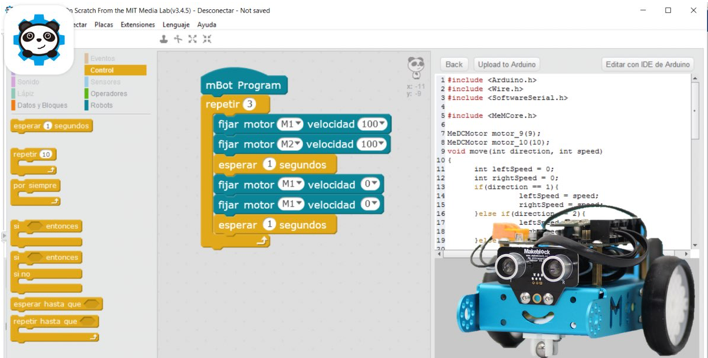
\includegraphics[width=1\textwidth]{images/software_mBlock.png}
  \caption{Software mBlock}
  \label{Software mBlock}
\end{figure}

\section{Diseño}

En la Figura 4.3. se muestra el diseño seguido para la integración del Mbot en la plataforma de Kibotics. La interacción típica entre robot físico, el navegador web en el ordenador del usuario y el servidor de Kibotics consta de los 10 pasos señalados en esa figura.
\\
\\
Gracias al diseño elegido no es necesario que el usuario instale nada en su ordenador ni en el robot para permitir su uso, por lo que el proceso de programación del robot se limitará a que una vez que el usuario ha realizado el programa se envíe al robot directamente.
\\
\begin{figure}[h!]
  \centering
    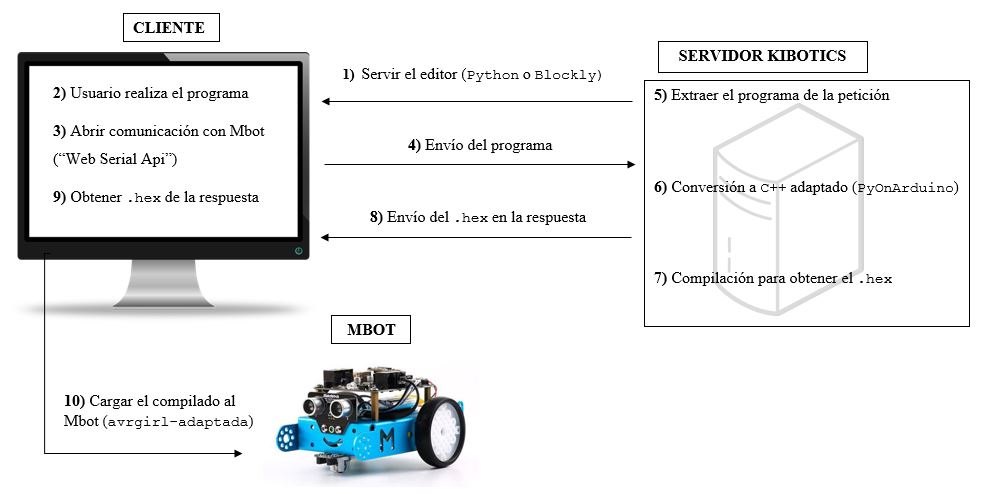
\includegraphics[width=1\textwidth]{images/infraestructura_mbot.png}
  \caption{Infraestructura seguida para la integración del Mbot}
  \label{Infraestructura seguida para la integración del Mbot}
\end{figure}
\\
En las secciones siguientes se detallarán cuáles son las interacciones necesarias entre el cliente y el servidor para permitir la carga del programa al Mbot y su ejecución a bordo.

\section{Lado Cliente}

Desde la parrilla principal de Kibotics se puede entrar a la unidad dedicada al Mbot, pudiendo elegir qué lenguaje de programación usar (\texttt{Python} o \texttt{Blockly}). Dentro de dicha unidad encontramos un apartado que proporciona las instrucciones necesarias para realizar un programa y enviárselo al Mbot real.

\subsection{Editor en el navegador web}

En la página web de Kibotics se proporciona un editor que le permitirá al usuario escribir en su propio navegador web el programa que será enviado al robot. Según la unidad elegida el editor estará orientado al lenguaje respectivo, \texttt{Blockly} o \texttt{Python}. Por ejemplo, la Figura 4.4 muestra un editor para \texttt{Blockly}.
\\
\begin{figure}[h!]
  \centering
    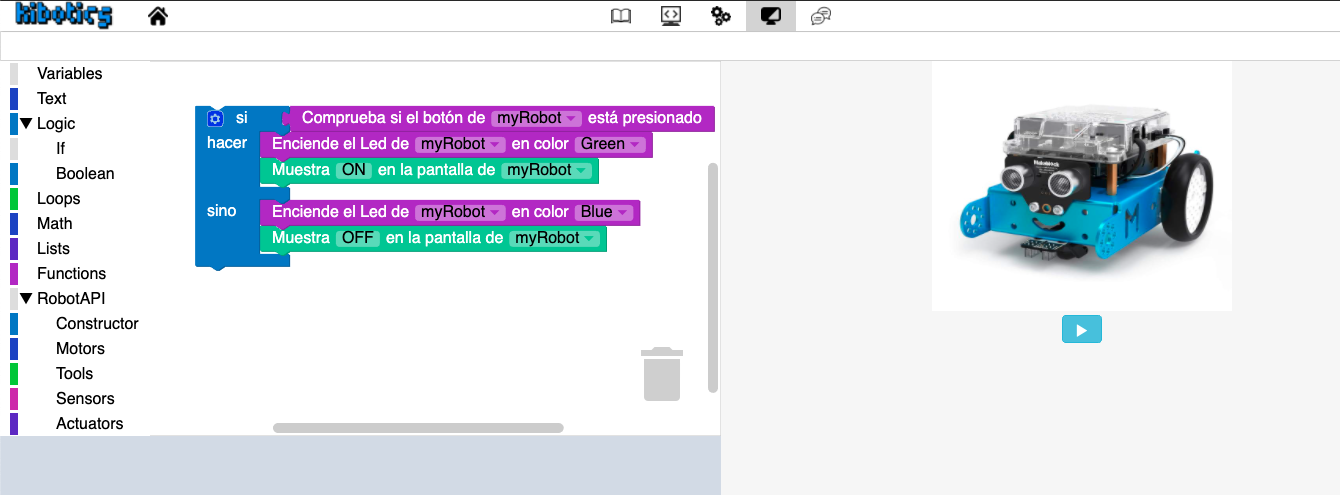
\includegraphics[width=1\textwidth]{images/editor_mbot.png}
  \caption{Editor Blockly para el Mbot }
  \label{Editor Blockly para el Mbot }
\end{figure}
\\

\subsection{Conexión con el Mbot vía USB}

Una vez que el usuario ha escrito el programa deseado y ha conectado físicamente el Mbot por USB a su ordenador, al pulsar el botón azul que se muestra en la Figura 4.4, se iniciará el proceso de envío.
\\
\\
En primer lugar, se abrirá una ventana que muestra los puertos del ordenador disponibles. Se debe seleccionar en el que se encuentra conectado el robot, que aparece nombrado como \textit{USB2.0Serial}. Esta acción permitirá abrir una comunicación entre el navegador y el robot (Fragmento 4.1). Esto es posible gracias al módulo \texttt{Web Serial API}, que proporciona una API al navegador capaz de interactuar con el puerto serie de la computadora.
\\
\begin{lstlisting}[frame=single,breaklines=true, label=Abrir conexión con el Mbot desde el navegador web por el puerto serie, caption=Abrir conexión con el Mbot desde el navegador web por el puerto serie, captionpos=b]  % Inicia el bloque de código
   document.addEventListener('DOMContentLoaded', () => {

      document.getElementById('uploadMbot').addEventListener('click', clickConnect);

   });

   async function clickConnect() {
      progress.style.width = '0%';
      alertError.style.visibility = 'hidden';
      //-- Si el puerto serie estaba ya abierto, cerrarlo
      if (portPrev) {
         await disconnect();
      }
      await connect();
      activeProgress.style.visibility = 'visible';
      progress.style.width = '25%';
      if(document.getElementById('uploadMbot').value == 'python'){
          send_code_to_mbot()
      }else{
          convert_and_send_code_to_mbot();
      }

   }

   async function connect() {
      portPrev = await navigator.serial.requestPort();

      await portPrev.open({ baudrate: 115200 });

   }
   async function disconnect() {
       // -- Cerrar el puerto serie
      await portPrev.close();
      portPrev = null;
   }
\end{lstlisting}


\subsection{Envío del código fuente al servidor}

Una vez abierta la comunicación USB de forma correcta, se procede a enviar el programa desde el navegador al servidor web Kibotics para su manipulación, como un \textit{query parameter} de una petición GET. Para este envío se utiliza la función \texttt{fetch()}, que está proporcionada por \texttt{JavaScript} (Fragmento 4.2).
\\
\begin{lstlisting}[frame=single,breaklines=true, label=Envío del programa desde el navegador al servidor web, caption=Envío del programa desde el navegador al servidor web, captionpos=b]
   function send_code_to_mbot() {
      var editor = ace.edit("ace");
      let code = editor.getValue();
      console.log(code);
      var enc = new TextEncoder();
      const message = {
         method: "GET"
       };
       url = '/get_python_to_arduino_binary?python_code=' + JSON.stringify(code);
       fetch(url, message)
             . . . . .
  
 }
\end{lstlisting}
Hay que tener en cuenta que si el programa está escrito en \texttt{Blockly}, debe convertirse previamente al lenguaje \texttt{Python} antes de enviarse, como puede verse en el fragmento 4.3.
\\
\begin{lstlisting}[frame=single,breaklines=true, label=Conversión de Blockly a Python, caption=Conversión de Blockly a Python, captionpos=b]
   var pythoncode = Blockly.Python.workspaceToCode(editor.ui);
\end{lstlisting}

\subsection{Recepción del ejecutable}

De la petición enviada al servidor por el navegador con el programa escrito por el usuario, se recibe una respuesta que contiene el programa ya compilado, ejecutable, para poder enviárselo a la microcontroladora a bordo del mBot.
\\
\\
La función \texttt{fetch()}, mencionada anteriormente, espera hasta recibir la contestación, pudiendo extraer  así el cuerpo de la respuesta, donde se encuentra el programa ejecutable.
\\
\begin{lstlisting}[frame=single,breaklines=true, label=Extracción del dato enviado en la respuesta, caption=Extracción del dato enviado en la respuesta, captionpos=b]
   fetch(url, message)
      .then(function(response) {
         if(response.ok){
            responseOk = true
         }else{
            responseOk = false
         }
           return response.text();
      })
      .then(function(data) {
        
         var dataBuffer = enc.encode(data);
           
      })
      .catch(function(err) {

         console.error(err);
       });

\end{lstlisting}


\subsection{Carga en el robot físico y ejecución a bordo}

Una vez extraído el código compilado, se procede a cargarlo en el robot. \texttt{Avrgirl-arduino}, una librería nodejs de código abierto, proporciona esa posibilidad de enviar el programa compilado a la microcontroladora, y es compatible con un gran número de placas (entre ellas \texttt{ArduinoUno}). Hemos utilizado esta librería adaptándola a nuestras necesidades para el proceso de carga.
\\
\begin{lstlisting}[frame=single,breaklines=true, label=Carga del compilado al Mbot, caption=Carga del compilado al Mbot, captionpos=b]
   . . . 
   
   .then(function(data) {

      if(responseOk){
         var dataBuffer = enc.encode(data);
         upload_to_mbot(dataBuffer)
         progress.style.width = '99%';
         alertError.style.visibility = 'hidden';
      }else{
         console.log("Fallo al compilar el programa")
         infoError.innerHTML = "Error"
         alertError.style.visibility = 'visible';
         activeProgress.style.visibility = 'hidden';
      }

   })
    . . . 
    
    function upload_to_mbot(dataBuffer){
       let avrgirl = new AvrgirlArduino({
          board: "uno"
       });

       avrgirl.flash(dataBuffer,(error) =>  {
          if (error) {
             console.error(error);
             portPrev = null;
             infoError.innerHTML = "Error!"
             alertError.style.visibility = 'visible';
             activeProgress.style.visibility = 'hidden';

          } else {
             console.info('done correctly.');
             portPrev = null
             alertError.style.visibility = 'hidden';
             activeProgress.style.visibility = 'hidden';
          }
      });
   }

\end{lstlisting}
Tras “quemar” el programa en el Mbot, este empezará automáticamente a ejecutar las instrucciones que le fueron programadas.

\section{Lado Servidor}

El servidor de Kibotics es el encargado de proporcionar al navegador las páginas que le permiten ir navegando por la web, y por lo tanto dirigirse a la unidad del Mbot. Pero también toma otro papel fundamental para el desarrollo del envío, ya que será el responsable de adaptar el código fuente que el usuario ha escrito, para que pueda ser entendido por la controladora del robot a la hora de realizarse la carga y ejecutarlo.

\subsection{Recepción del código fuente}

Una vez que el usuario realizó su programa y pulsó en enviar, el navegador le envía al servidor el código fuente escrito para que este lo adapte. Por lo que el servidor tendrá que extraer el código (Fragmento 4.6), que se encuentra en un \textit{query parameter} de la URL.
\\
\begin{lstlisting}[frame=single,breaklines=true, label=Extracción del programa en el servidor, caption=Extracción programa en el servidor, captionpos=b]
   def get_python_to_arduino_code_binary(request):
      . . . .
      python_code = json.loads(request.GET.get('python_code', None))
      . . . .

\end{lstlisting}

\subsection{Conversión a lenguaje Arduino/C++}

El programa extraído en el servidor es lenguaje \texttt{Python}, pero el Mbot, basado en \texttt{Arduino}, no entiende este lenguaje. El lenguaje de alto nivel que usa \texttt{Arduino}, para posteriormente generar el compilado que entiende, es un C++ adaptado, por lo que se debe traducir desde \texttt{Python}. Esto es posible gracias a la librería \texttt{PyOnArduino}, la cual proporciona los mecanismos necesarios para esa traducción y conversión de un fichero.py (extensión para \texttt{Python}) a .ino (extensión para \texttt{Arduino}).
\\
\begin{lstlisting}[frame=single,breaklines=true, label=Traducción de lenguaje Python a Arduino, caption=Traducción de lenguaje Python a Arduino, captionpos=b]
   . . .    
    parsed_file = ast.parse(code)
    translator.robot = 'MBot'
    translator.robot_architecture = ''
    translator.vars.Variables()
    translator.vars.halduino_directory = py_to_arduino_path + 'HALduino/halduino'
    translator.TranslatorVisitor().visit(parsed_file)
    translator.create_setup()
    translator.variables_manager = translator.create_variables_manager(file=py_to_arduino_path + 'HALduino/variablesManager.ino')
    translator.create_output('output-file.ino')
    translator.create_makefile('MBot', py_to_arduino_path + 'makefiles/')
    . . .


\end{lstlisting}


\subsection{Compilación cruzada}

Una vez conseguido el código en Arduino/C++, se debe compilar para obtener el fichero .hex que contiene las instrucciones traducidas a hexadecimal ya ejecutables por la microcontroladora. Esta compilación se lleva a cabo utilizando \texttt{avrdude}, una herramienta que permite la programación de chips AVR y que puede ser llamada por la línea de comandos. 
\\
\begin{lstlisting}[frame=single,breaklines=true, label=Compilado y obtención del .hex, caption=Compilado y obtención del .hex, captionpos=b]
def create_mbot_binary():
    shutil.copyfile(os.path.join(settings.BASE_DIR, 'kibotics-drivers/mbot/avrdude'), './avrdude')
    shutil.copyfile(os.path.join(settings.BASE_DIR, 'kibotics-drivers/mbot/libftdi1.so'), './libftdi.so')
    shutil.copyfile(os.path.join(settings.BASE_DIR, 'kibotics-drivers/mbot/libreadline.so'), './libreadline.so.6')
    shutil.copyfile(os.path.join(settings.BASE_DIR, 'kibotics-drivers/mbot/avrdude.conf'), './avrdude.conf')
    shutil.copytree(os.path.join(settings.BASE_DIR, 'kibotics-drivers/mbot/arduino-1.8.10/'), 'arduino/')
    call(['make'])
    exercise_dir = './'
    # Extraemos el binario
    f_binary = open(exercise_dir + 'build-uno/output.hex', 'r')
    binary = f_binary.read()
    f_binary.close()
    return binary
\end{lstlisting}

\subsection{Envío del ejecutable}

Tras la compilación del programa en el servidor, obtenemos el .hex que será enviado como respuesta al navegador, para que pueda ser cargado al robot que está junto al usuario.
\\
\begin{lstlisting}[frame=single,breaklines=true, label=Respuesta a la petición que envió el navegador, caption=Respuesta a la petición que envió el navegador, captionpos=b]
    . . .
    binary = create_mbot_binary()

    response = HttpResponse(binary, content_type='text/plain')
    response['Content-Length'] = len(response.content)
    return response
\end{lstlisting}

\section{Validación experimental}

En las secciones anteriores no se ha mencionado en ningún momento para qué sistema operativo era compatible todo el proceso de envío, y es aquí donde recae una de las principales ventajas de este desarrollo. Al tratarse de una tecnología web de lado del navegador proporciona compatibilidad para cualquier sistema operativo que disponga de un navegador basado en \texttt{Chromiun} (Google Chrome, Opera, Edge), ya que actualmente \texttt{Web Serial API} solo está disponible para ellos. Con este diseño se consigue un soporte del mBot multiplataforma, que funciona con independencia del sistema operativo del usuario de Kibotics.
\\
\\
Además, al no necesitar una instalación previa de dependencias o programas por parte del usuario, su usabilidad es más sencilla. Esto es muy importante de cara al uso de la plataforma, ya que al estar orientada a alumnos de baja edad, es necesario que el proceso sea lo más simple posible.
\\
\\
La principal desventaja es que, actualmente, \texttt{Web Serial API}  está en fase de experimentación en los navegadores \texttt{Chromiun}, por lo que necesita ser activada con un proceso previo. Para ello, para activarla por ejemplo en Chrome, debemos escribir en el navegador Chrome \textit{“chrome://flags”} y habilitar el flag \textit{“Experimental web Plataform features”}.
\\ 
\\
La integración del Mbot ha sido probada en diferentes sistemas operativos, verificando el correcto funcionamiento en todos ellos (\texttt{Ubuntu 18.04}, \texttt{Ubuntu 16.04}, \texttt{Windows 10},  \texttt{Windows 8},  \texttt{MacOS Mojave Versión 10.14.6}).
\\
\\
Por último, se han grabado una serie de vídeos donde se puede observar un ejemplo de realización de un programa y envío al Mbot desde la plataforma Kibotics para los principales sistemas operativos:
\begin{itemize}
	\item \textbf {\texttt{MacOS}:} \textit{\url{https://www.youtube.com/watch?v=UyNa9R-L0Ps}}
	\item \textbf{\texttt{Linux}:} \textit{\url{https://youtu.be/1jyvoN5ZRxQ}}
	\item \textbf {\texttt{Windows}:} \textit{\url{https://youtu.be/4Wq4kMRUeIc}}
\end{itemize}
En la figura 4.5 se muestran unos fotogramas del vídeo de ejemplo para \texttt{MacOS}. En ella se observa que el primer paso es realizar el programa deseado. Una vez creado, al pulsar en el botón de envío, se abre el panel para conectarnos con el puerto serie del robot. Finalmente, una vez conectados al robot, el programa es cargado en él, terminando así el proceso de envío. Este proceso sería el mismo para \texttt{Windows} y \texttt{Linux}.

\begin{figure}[h!]
  \centering
    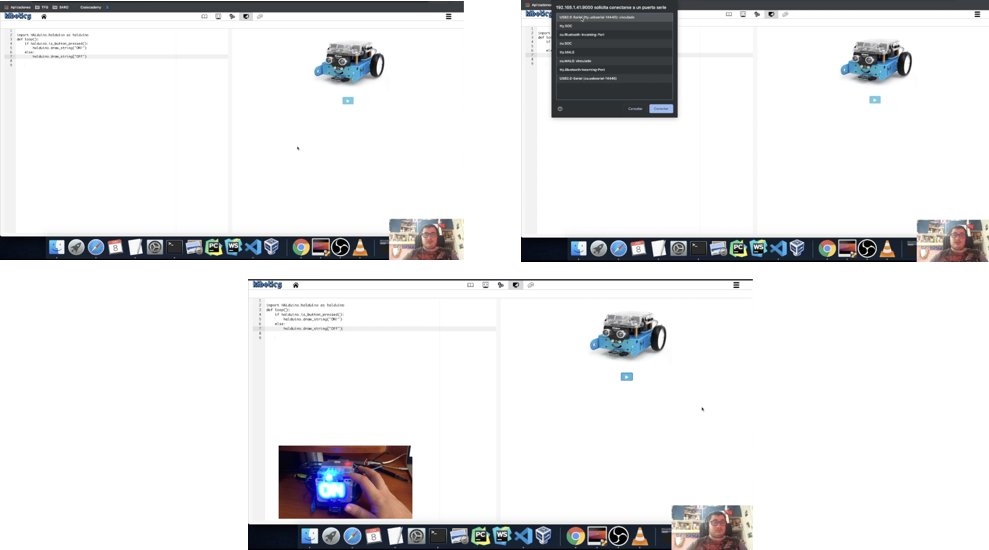
\includegraphics[width=1\textwidth]{images/fotogramas_mbot.png}
  \caption{Fotogramas del vídeo de ejemplo de envío para el Mbot en MacOS}
  \label{Fotogramas del vídeo de ejemplo de envío para el Mbot en MacOS}
\end{figure}






%###############################################################################
%###################### Tello ####################################################
%###############################################################################


\chapter{Integración del dron Tello}

En este capítulo se describe el desarrollo realizado para poder programar el dron Tello. A diferencia del Mbot, donde el proceso era similar para cualquier sistema operativo, en este caso el proceso va a variar.

\section{Características del drone Tello}

Tello es un mini dron distribuido por la empresa Ryze Technology \footnote{\url{https://www.ryzerobotics.com/es}} (Figura 5.1). Debido a la facilidad de su uso, está destinado tanto a niños como a adultos que quieran aprender a utilizar drones. Puede alcanzar una velocidad de hasta 28 km/h, su radio de control abarca hasta los 100 metros y su señal de vídeo se transmite a una frecuencia de 2,4Ghz. Posee una unidad procesadora de Intel, un barómetro para controlar de altura, motores de tipo escobilla y una cámara de 720p. Además, sus hélices están protegidas y es resistente a las caídas.
\\
\begin{figure}[h!]
  \centering
    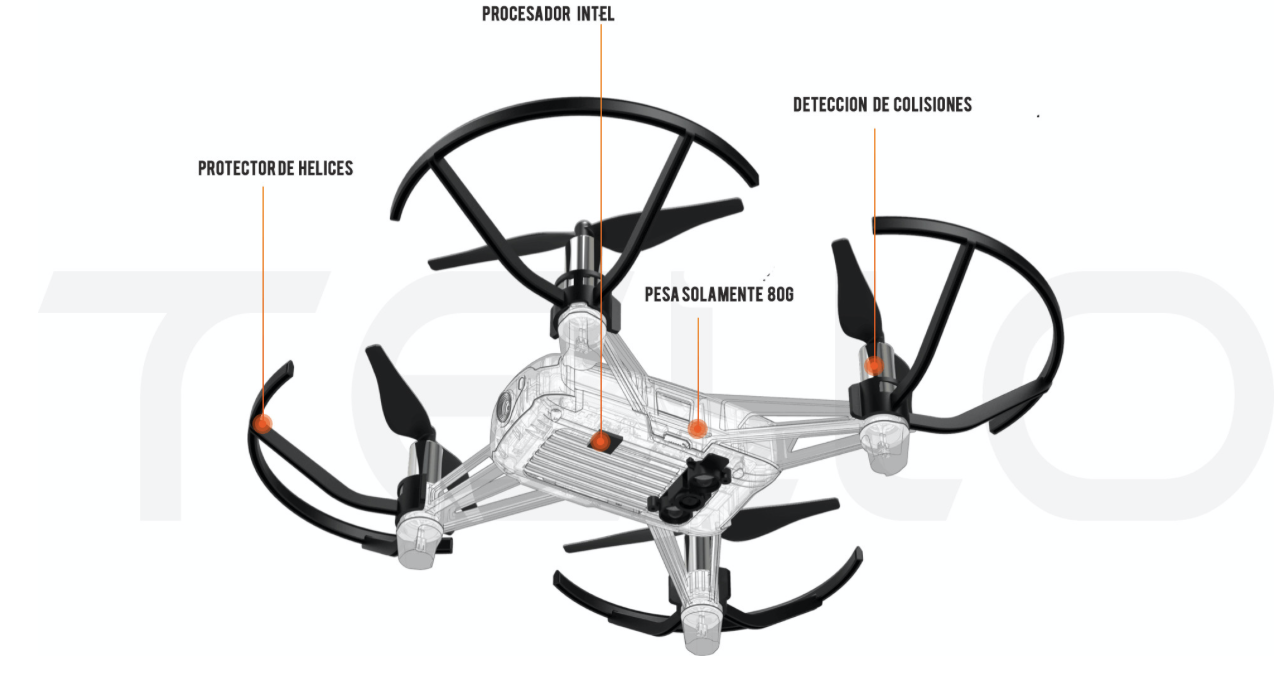
\includegraphics[width=0.75\textwidth]{images/partes_dron_tello.png}
  \caption{Esquema del dron Tello}
  \label{Esquema del dron Tello}
\end{figure}
\\
Entre sus puntos fuertes destacan su gran estabilidad durante el vuelo y que utiliza un sistema de posicionamiento por visión (VPS). El sistema VPS utiliza un mínimo de dos cámaras para medir la distancia al suelo y la posición a la que se encuentra, compensando así los cambios en la posición que puedan darse (Castro, 2019).
\\
\\
Existen una variedad de software que permiten programar al Tello, entre los que destacan(Figura 5.2).
\begin{itemize}
	\item Tello EDU App, es una aplicación diseñada para móviles o tables (iOS y Android), creada por la propia empresa que distribuye a este dron (RYZE Technology), que permite programarle utilizando bloques. Además incluye una opción para programar a un dron Tello simulado.
	\item El IDE (\textit{Integrated Development Environment}) de Scratch ofrece la posibilidad de programar a este dron utilizando este lenguaje, aunque requiere para su uso de instalaciones previas en el ordenador del usuario.
	\item DroneBlocks además de permitir programar el Tello, ofrece la posibilidad de utilizar otros drones (Phantom 3, Phantom 4, Mavic Pro, Mavic Air, Spark). Utiliza también un lenguaje de bloques basado en \texttt{Scratch} y está disponible en iOS App Store,  Google Play Store y Chrome App Store.
\end{itemize}
\begin{figure}[h!]
  \centering
    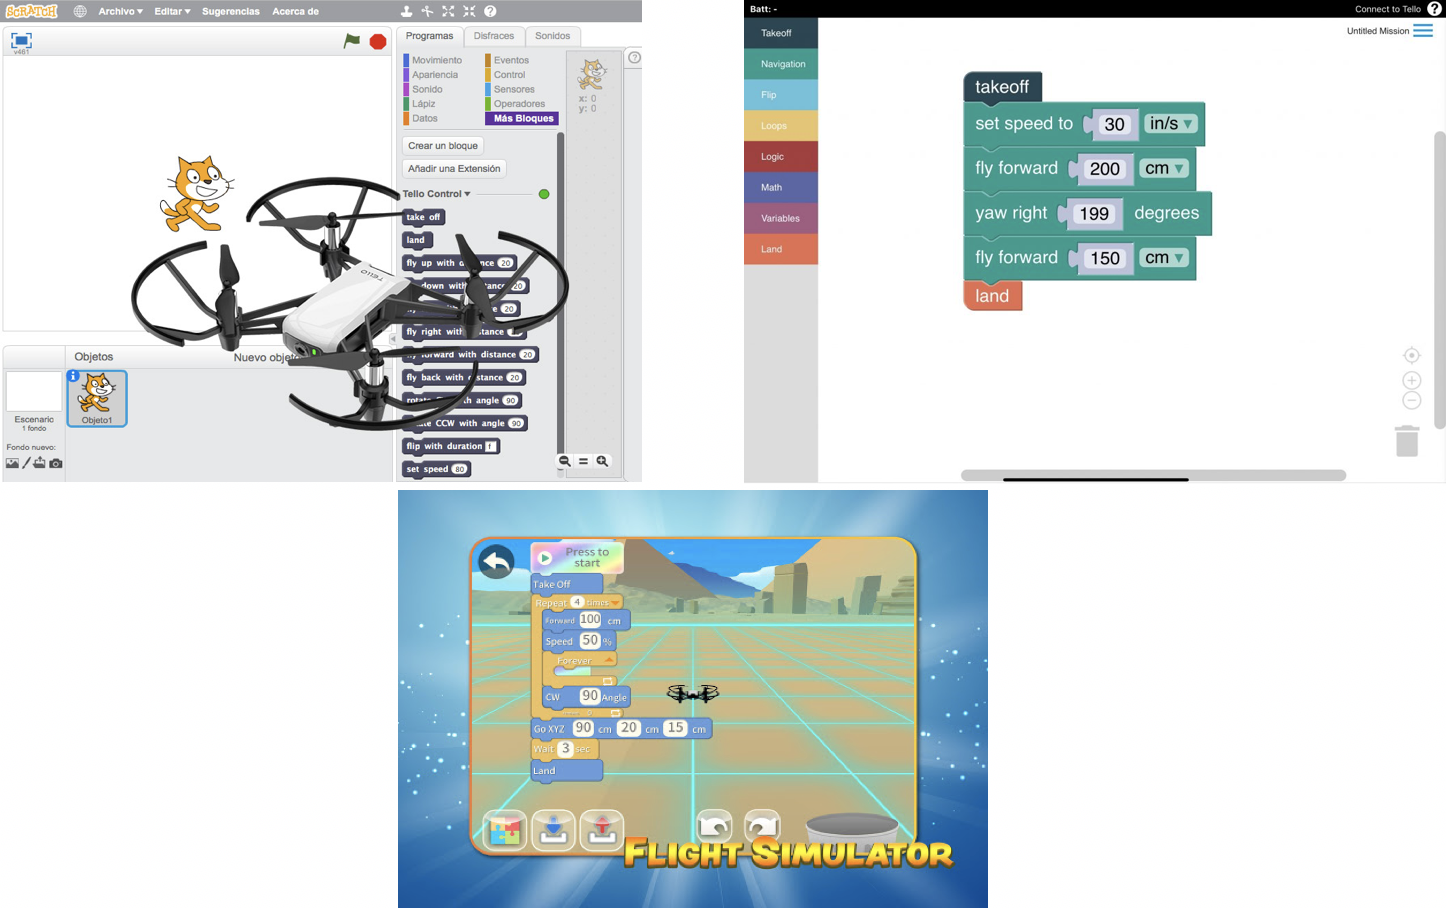
\includegraphics[width=0.8\textwidth]{images/software_tello_ide.png}
  \caption{IDE de Arduino (arriba a la izquiera), DroneBlocks (arriba a la derecha) y Tello EDU App (abajo)}
  \label{IDE de Arduino, DroneBlocks y Tello EDU App}
\end{figure}

\section{Diseño}

En la Figura 5.3, se muestra cuál es la arquitectura necesaria para conseguir el envío del programa al dron Tello real desde la plataforma Kibotics.
\\
\\
Para el Mbot no se requería ninguna instalación y, además, el proceso de envío del programa era el mismo para los diferentes sistemas operativos. En el caso del Tello, existen peculiaridades para los diferentes sistemas operativos al no tener control sobre la controladora que posee el robot y al necesitar un \textit{proxy} intermediario. Aunque en el robot no es necesario instalar nada, si que se necesitarán unos requisitos previos para los ordenadores que sean \texttt{Windows} y \texttt{MacOS}.
\\
\begin{figure}[h!]
  \centering
    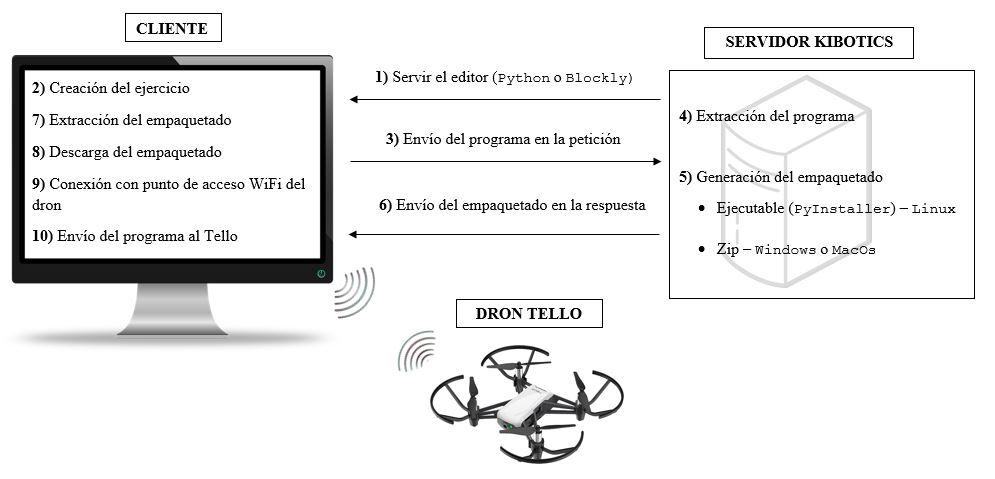
\includegraphics[width=1\textwidth]{images/infraestructura_tello.png}
  \caption{Arquitectura del desarrollo para el Tello}
  \label{Arquitectura del desarrollo para el Tello}
\end{figure}
\\
A continuación hablaremos en detalle sobre estos 10 pasos necesarios para conseguir la integración del Tello en Kibotics en los sistemas operativos \texttt{Linux}, \texttt{Windows} y \texttt{MacOS}.

\section{Lado cliente}

En la parrilla de Kibotics se encuentran dos unidades dedicadas al dron Tello, una dedicada a su programación utilizando \texttt{Python} y otra con \texttt{Blockly}. En la unidad se encuentra una sección que proporciona información sobre los requisitos para este robot y cómo utilizarlo. 


\subsection{Preparación del anfitrión}

Para \texttt{MacOS} y \texttt{Windows} es indispensable que el usuario tenga instalado \texttt{Python} en su versión 2.7 y los \textit{drivers} necesarios para el uso del Tello. La empresa DJI posee un repositorio en GitHub \footnote{\url{https://github.com/dji-sdk/Tello-Python}} en el que se facilitan instaladores para su uso en los diferentes sistemas operativos. Por lo que el usuario tendría que instalar estos requisitos. Aunque para el caso de \texttt{MacOS}, en la página de información de la unidad del Tello se le proporciona a el usuario un ejecutable (Fragmento 5.1) que permitirá instalar todas las dependencias necesarias para su uso.
\\
\begin{lstlisting}[frame=single,breaklines=true, label=Ejecutable de instalación para MacOS, caption=Ejecutable de instalación para MacOS,  captionpos=b]
   #!/bin/bash

   ######### Requirements #########

   env=~/.virtualenvs/tello-env
   if [ -d $env ];
   then
      source ~/.virtualenvs/tello-env/bin/activate
   else
      if ! type "pip" > /dev/null; then
         sudo easy_install pip
       fi
       if ! type "brew" > /dev/null; then
          /usr/bin/ruby -e "$(curl -fsSL https://raw.githubusercontent.com/Homebrew/install/master/install)"  
          brew update
       fi
       sudo brew install cmake
       sudo brew install boost
       sudo brew install boost-python
       sudo brew install ffmpeg
       sudo brew install tcl-tk
    
       mkdir ~/.virtualenvs
       pip install virtualenv
       virtualenv ~/.virtualenvs/tello-env --python=python2.7
       source ~/.virtualenvs/tello-env/bin/activate
       pip install SimpleWebSocketServer
       pip install numpy
       pip install matplotlib
       pip install opencv-python==3.1.0.1
   fi
\end{lstlisting}
En \texttt{Linux}, sin embargo, no es necesaria ninguna instalación previa para poder utilizar este dron. Esto es gracias a \texttt{PyInstaller}, una librería de \texttt{Python}, y a que el servidor de Kibotics se encuentra en una máquina \texttt{Linux}. En las próximas secciones se profundizará en este aspecto.

\subsection{Editor en el navegador web}

En la página web de cada unidad se tiene también un editor (\texttt{Python} o \texttt{Blockly}), adaptado a la programación del Tello, donde el usuario podrá escribir su programa. El aspecto es similar al de los utilizados para el Mbot. 
\\
\\
Una vez que el usuario ha desarrollado el programa, debería pulsar el botín azul llamado “Ejecutar en Tello” (Figura 5.4) para iniciar el proceso de envío, que varía dependiendo del sistema operativo utilizado por el usuario de Kibotics.
\\
\begin{figure}[h!]
  \centering
    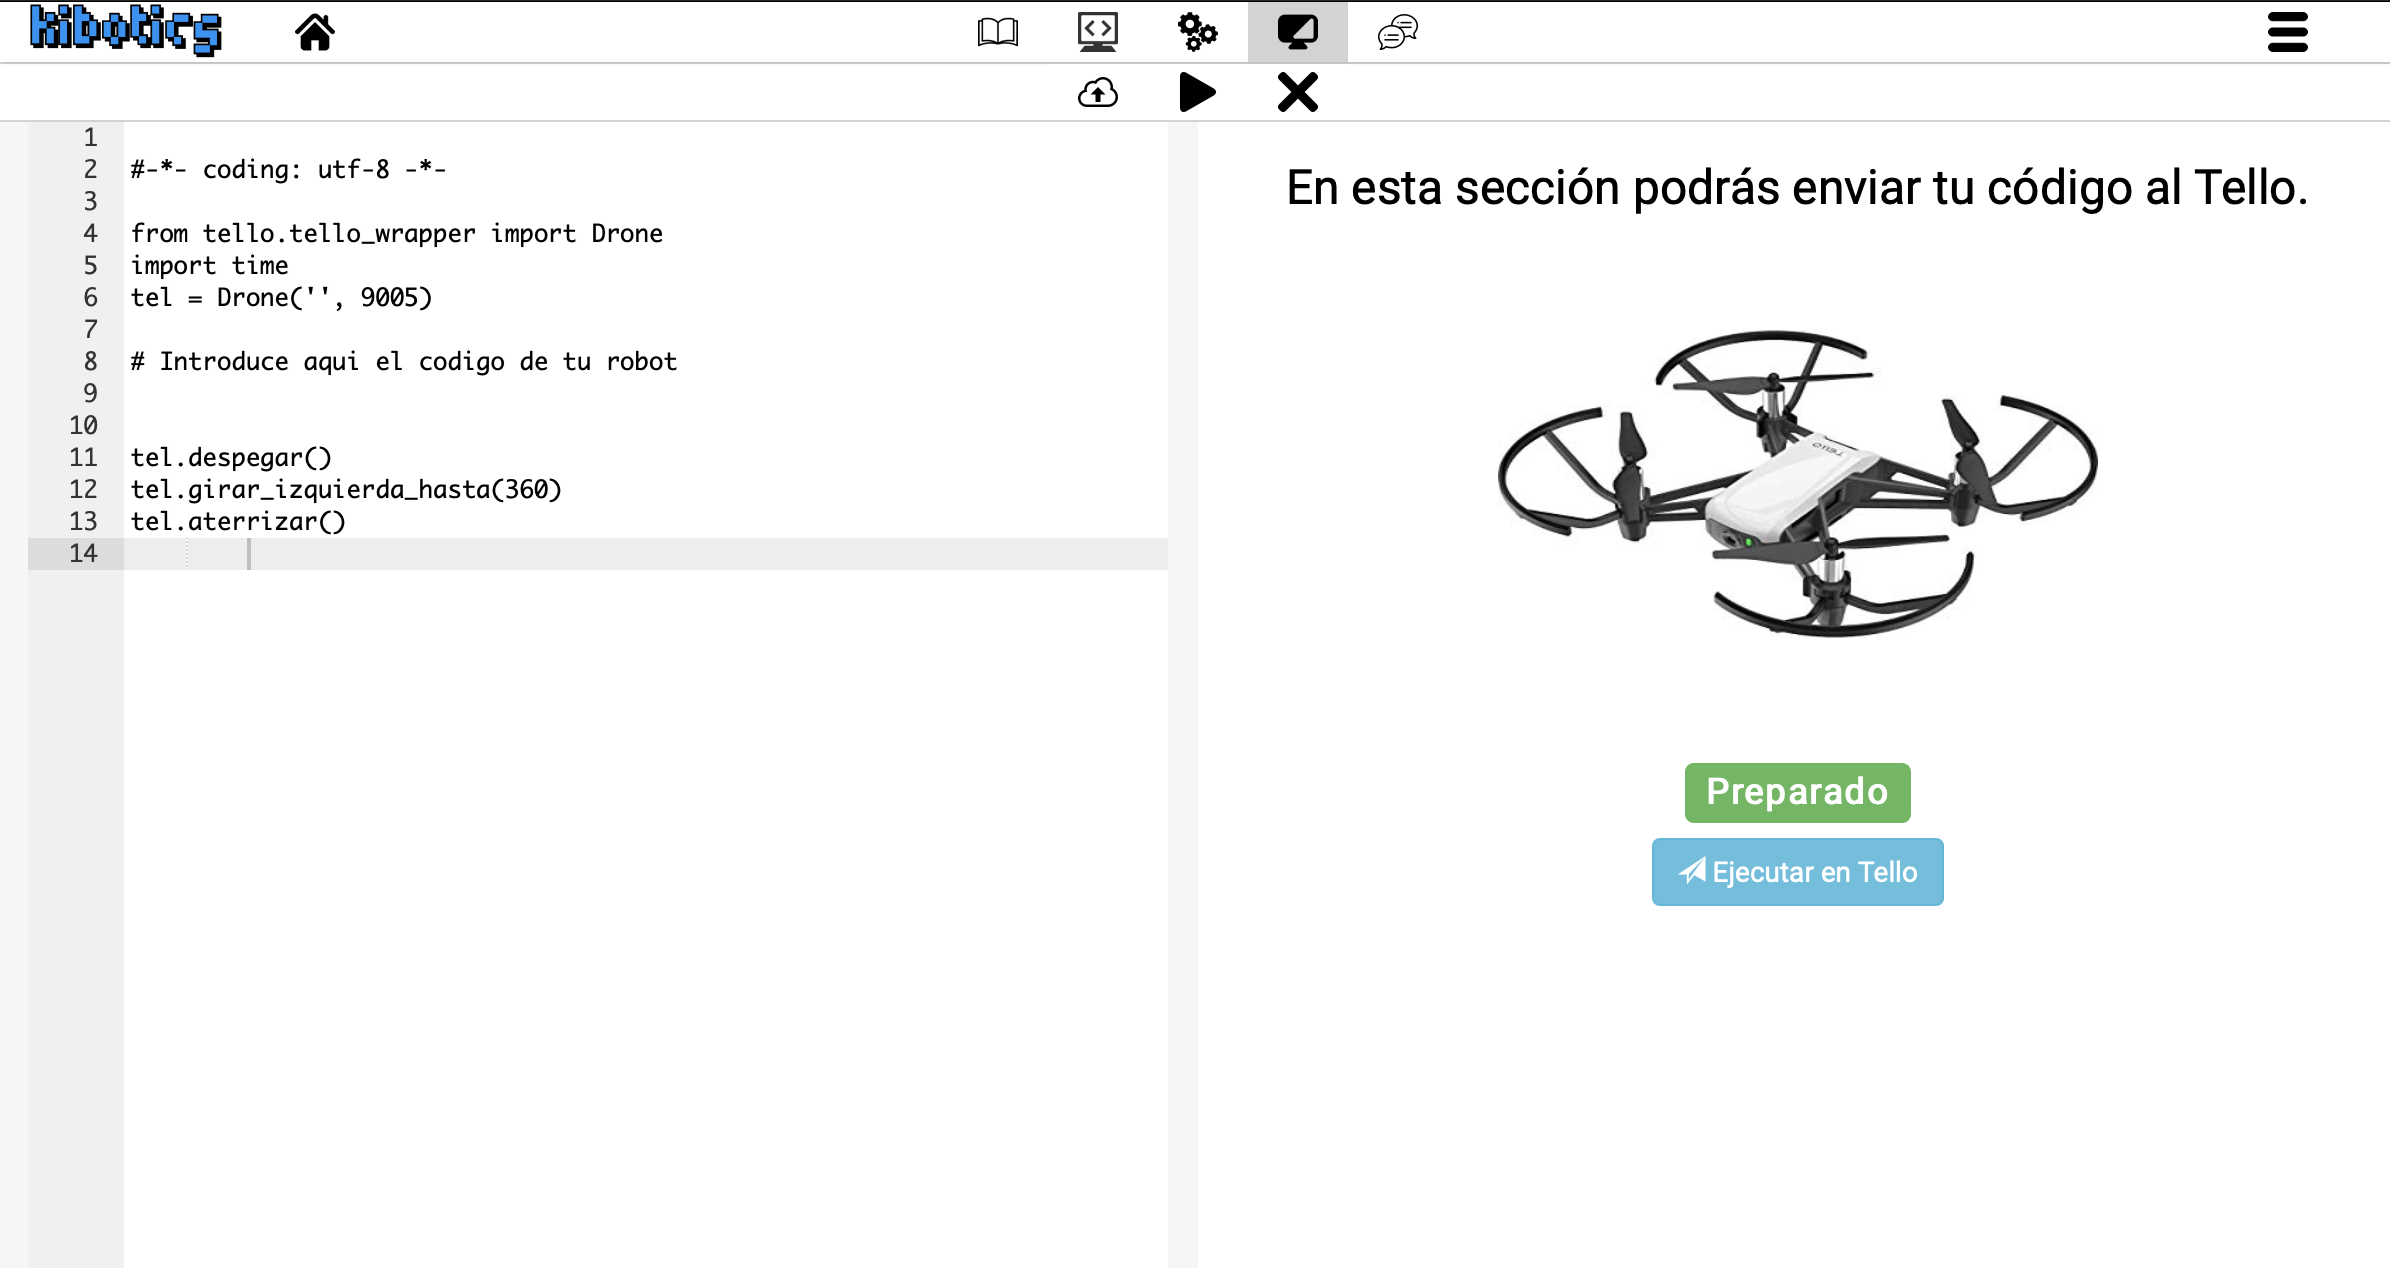
\includegraphics[width=0.9\textwidth]{images/editor_tello.png}
  \caption{Editor para programar el dron Tello en Python}
  \label{Editor para programar el dron Tello en Python}
\end{figure}


\subsection{Envío del código fuente al servidor}

Una vez iniciado el proceso de envío, el primer paso es enviar el código escrito por el usuario desde el navegador web al servidor de Kibotics, para generar el ejecutable que funciona con el Tello real. 
\\
\\
Se extrae el código escrito en el editor y se envía desde el navegador al servidor en un \textit{query parameter} de una petición GET (Fragmento 5.2).
\\
\begin{lstlisting}[frame=single,breaklines=true, label=Envío del programa desde el navegador al servidor", caption=Envío del programa desde el navegador al servidor,captionpos=b]
   
   function send_code_tello() {
      var editor = ace.edit("ace");
      let code = editor.getValue();
      console.log(code);
      const message = {
         method: "GET"
       };
       var = url = '/get_code_to_tello?python_code=' + JSON.stringify(code);
       fetch(url, message)
             . . . . .
  }
\end{lstlisting}



\subsection{Recepción del ejecutable}

El navegador queda a la espera de recibir la respuesta a la petición que envió al servidor. Y tras obtener esta respuesta, extrae un ejecutable en el caso de que se use una máquina \texttt{Linux}, o un fichero comprimido en el caso de usar \texttt{Windows} o \texttt{MacOS}, que preparó el servidor y que permitirá realizar la ejecución del programa.  Posteriormente, el fichero extraído se descargará en el ordenador de usuario.
\\
\begin{lstlisting}[frame=single,breaklines=true, label=Extracción del empaquetado, caption=Extracción empaquetado,  captionpos=b]
   . . .
   
   var = url = '/get_code_to_tello?python_code=' + JSON.stringify(code);
   fetch(url, message)
      .then(response => {
         ld.style.display = "none";
         if (response.ok) {
            download_executable(response);
         } else {
            console.error("Bad Response");
         }
      })
     .catch(err => console.error(err));
   }
   
   function downloadExecutable(response) {
      response.blob().then(blob => {
         var down = document.createElement("down");
         document.body.appendChild(down);
         down.style = "display: none";
         url = window.URL.createObjectURL(blob);
         down.href = url;
         down.download = 'tello_code';
         down.click();
         window.URL.revokeObjectURL(url)
      })
   }
\end{lstlisting}

\subsection{Conexión con el drone}

Para poder ejecutar el programa y que conecte con el Tello, necesitamos estar conectados con él. El dron, una vez encendido, crea un punto de acceso \textit{WiFi}, que tendrá el nombre Tello seguido de un número (Figura 5.5), al que se tiene que conectar el usuario. Necesitamos esta pasarela para comunicarnos con él.
\\
\begin{figure}[h!]
	\centering
    	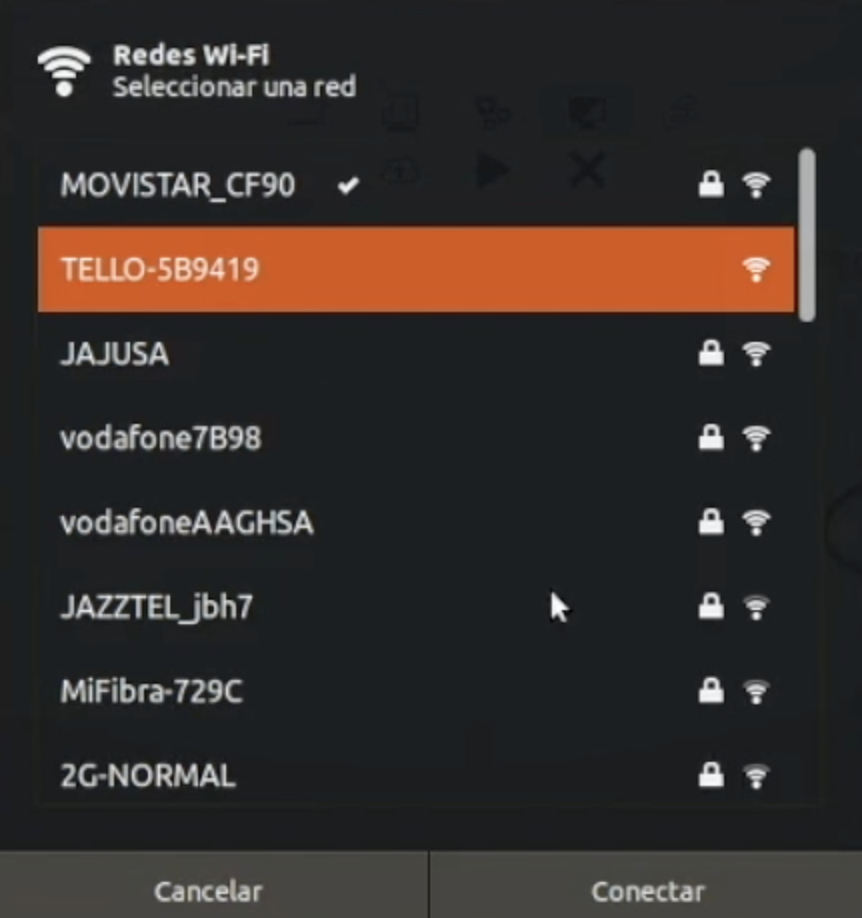
\includegraphics[width=0.4\textwidth]{images/seleccionar_wifi_tello.png}
  	\caption{Conectarse al punto de acceso WiFi emitido por el dron}
  	\label{Conectarse al punto de acceso WiFi emitido por el dron}
\end{figure}


\subsection{Ejecución}


El fichero descargado en el ordenador permitirá ejecutar el programa y que conecte con el Tello, como este fichero es diferente para cada uno de los sistemas operativos, el proceso que hay que seguir para ejecutarlo no es el mismo. A continuación se describe cual es el proceso de ejecución para cada uno de los sistemas operativos:
\begin{itemize}
	\item \textbf{Ejecución Linux.} 
		\begin{enumerate}
			\item Se descargará un ejecutable en el ordenador anfitrión. Este ejecutable es autocontenido, incluye el intérprete de \texttt{Python}, el código del usuario, el driver del Tello y todas las bibliotecas necesarias.
			\item Dirigirse al directorio donde se descargo, darle permisos de ejecución y ejecutarlo (Fragmento 5.4).
			\\
			\begin{lstlisting}[frame=single,breaklines=true, label=Comandos para ejecución del envío en MacOS, caption=Comandos para ejecución del envío en MacOS,  captionpos=b]
		chmod +x send_code.sh &&
		./send_code.sh
			\end{lstlisting}
		\end{enumerate}
	\item \textbf{Ejecución en Windows.} 
		\begin{enumerate}
			\item Se descargará un fichero comprimido. Este fichero comprimido contiene el código del usuario y todas las bibliotecas necesarias, no contiene el intérprete de \texttt{Python}.
			\item Descomprimir el fichero y dirigirse a  directorio extraído.
			\\
			\begin{figure}[h!]
 			 	\centering
    				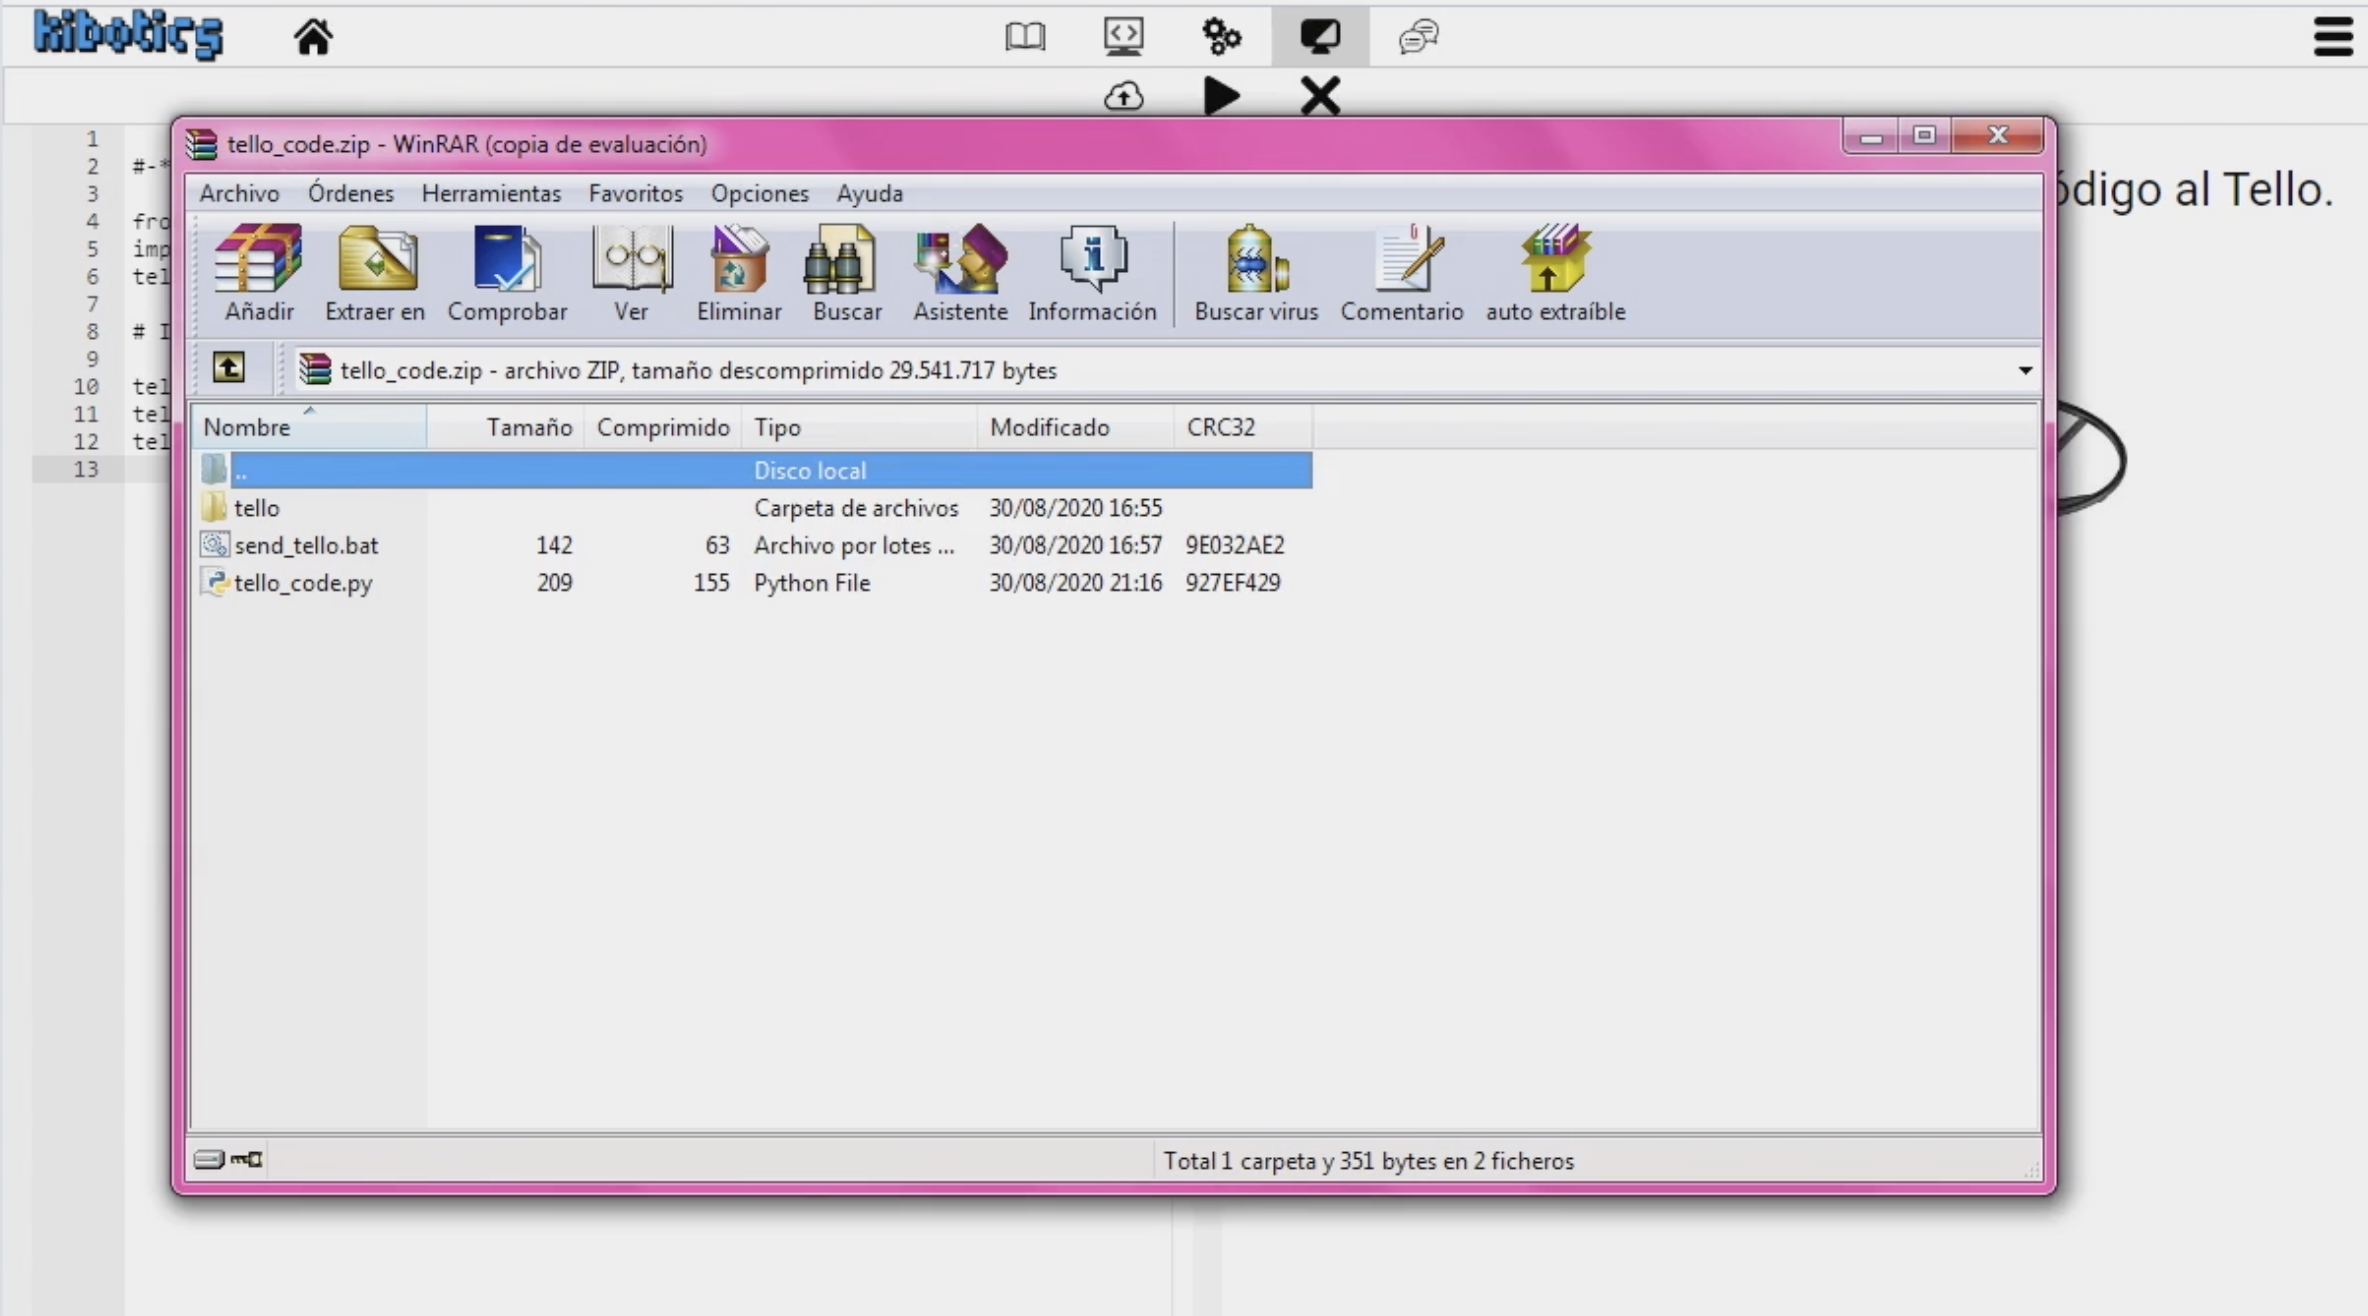
\includegraphics[width=1\textwidth]{images/descarga_windows_tello.png}
  				\caption{Descompresión en Windows}
  				\label{Descompresión en Windows}
			\end{figure}
			\item Haciendo doble “\textit{click}” en el ejecutable send\_tello.bat, el programa se ejecutará y establecerá conexión con el Tello.
		\end{enumerate}
	\item \textbf{Ejecución en MacOS.}
		\begin{enumerate}
			\item Se descargará un fichero comprimido. Este fichero comprimido contiene el código del usuario y todas las bibliotecas necesarias, no contiene el intérprete de \texttt{Python}.
			\item Descomprimir el fichero y dirigirse a  directorio extraído.
			\item Dentro del directorio se encuentra un fichero ejecutable llamado "send\_code.sh", al que se tendrá que dar permisos de ejecución y, posteriormente, lanzarlo para ejecutar el programa y que conecte con el dron (Fragmento 5.5).			
			\\
			\begin{lstlisting}[frame=single,breaklines=true, label=Comandos para ejecución del envío en MacOS, caption=Comandos para ejecución del envío en MacOS,  captionpos=b]
		chmod +x send_code.sh &&
		./send_code.sh
			\end{lstlisting}
		\end{enumerate}
\end{itemize}



\section{Lado servidor}

Como ocurría en el Mbot, el servidor de Kibotics, además de ser el responsable de servir las páginas, también es el encargado de adaptar el código que ha escrito el usuario para que el programa pueda ser ejecutado. 
\\
\\
En este caso, la adaptación consiste en realizar un empaquetado que será devuelto al navegador. En los siguientes apartados se describen los pasos seguidos para conseguirlo.

\subsection{Recepción del código fuente}

Una vez que el usuario ha escrito el programa y se ha iniciado el proceso de envío, el navegador envía el código creado por el usuario al servidor. Este extrae dicho código del \textit{query parameter} de la petición recibida (Fragmento 5.6). 
\\
\begin{lstlisting}[frame=single,breaklines=true, label=Extracción del programa fuente en el servidor, caption=Extracción del programa fuente en el servidor, captionpos=b]
   def get_code_to_tello(request):
      . . . .
      python_code = json.loads(request.GET.get('python_code', None))
      . . . .

\end{lstlisting}


\subsection{Empaquetado}

El dron Tello entiende el lenguaje \texttt{Python}, y como el código extraído ya se encuentra escrito en este lenguaje, no será necesarío realizar ninguna conversión. Por lo tanto, una vez extraído el código se procede a su empaquetado, que será diferente en función del sistema operativo utilizado por el usuario.
\\
\begin{itemize}
	\item \textit{\textbf{Linux}}. El empaquetado consistirá en realizar un ejecutable que contenga todas las dependencias necesarias para el envío. Esto es posible gracias a una librería de \texttt{Python} llamada \texttt{PyInstaller}, un módulo que permite empaquetar ficheros \texttt{Python}, generando así un ejecutable autocontenido e incluyendo dentro del propio ejecutable el intérprete de \texttt{Python}. \texttt{PyInstaller} no permite una "\ compilación cruzada", es decir, si este empaquetado se realiza en una máquina \texttt{Linux}, el ejecutable solo podrá utilizarse en una máquina \texttt{Linux}. Debido a esto, la integración para el dron Tello varía según el sistema operativo; como el servidor de Kibotics está alojado en una máquina \texttt{Linux}, solo los usuarios de \texttt{Linux} se beneficiarán de esta utilidad.
\begin{lstlisting}[frame=single,breaklines=true, label=Creación ejecutable con PyInstaller, caption=Creación ejecutable con PyInstaller,  captionpos=b]
   def create_executable_with_pyinstaller(exercice_path):
    		      
   	call(". kibotics-drivers/tello/tello_env/bin/activate; pyinstaller -F --distpath " +
      	exercice_path + "dist --workpath " + exercice_path + "build --specpath " + exercice_path + " --clean " + exercice_path +
      	"tello_code.py", shell=True)
      . . . 
\end{lstlisting}
	
	
	\item \textit{\textbf{Windows y MacOS}}. El proceso es similar en ambos, pero diferente al caso anterior. Se empaqueta el programa con el directorio que engloba todas las librerías y las dependencias necesarias y que, además, contiene el ejecutable .bat (en \texttt{Windows}) o .sh (en \texttt{MacOS}) que se encargará del envío (Fragmento 5.8). Además la única diferencia entre ambos, es que al necesitar dependencias especificas de cada sistema operativo(el driver nativo del Tello en \texttt{Windows} es distinto del driver nativo del Tello en \texttt{MacOS}) , se utilizan directorios diferentes en el empaquetado.
	\\
\begin{lstlisting}[frame=single,breaklines=true, label=Creación empaquetado en Windows y MacOS, caption=Creación empaquetado y respuesta en Windows y MacOS,  captionpos=b]
   if operative_system == 'Mac':
        shutil.move(exercise_dir + "tello_code.py", os.getcwd() + "/kibotics-drivers/tello/MacOS")
        shutil.make_archive('output-tello-mac', 'zip', os.getcwd() + "/kibotics-drivers/tello/MacOS")

    elif operative_system == 'Windows':
        shutil.move(exercise_dir + "tello_code.py", os.getcwd() + "/kibotics-drivers/tello/Windows")
        shutil.make_archive('output-tello-windows', 'zip', os.getcwd() + "/kibotics-drivers/tello/Windows")

\end{lstlisting}	

\end{itemize}


\subsection{Envío del empaquetado}

Una vez generado el empaquetado, ejecutable en \texttt{Linux} y fichero comprimido en \texttt{MacOS} y \texttt{Windows}, se devuelve al navegador en la respuesta a la petición que envió. Esto permitirá que sea descargado en el ordenador del usuario y pueda ejecutarlo, consiguiendo así que el programa ejecute con el dron Tello.
	\\
\begin{lstlisting}[frame=single,breaklines=true, label=Respuesta a la petición para Linux, caption=Respuesta a la petición para Linux,  captionpos=b]
   create_executable_with_pyinstaller(exercice_path)
   response = FileResponse(open(exercice_path + "dist/tello_code", 'rb'), content_type='application/octet-stream')
   shutil.rmtree(exercise_dir + "dist/")
   shutil.rmtree(exercise_dir + "build/")
   os.remove(exercise_dir + "tello_code.spec")
\end{lstlisting}
\begin{lstlisting}[frame=single,breaklines=true, label=Respuesta con empaquetado en Windows y MacOS, caption=Creación empaquetado y respuesta en Windows y MacOS,  captionpos=b]
   if operative_system == 'Mac':
        . . . 
        with open('output-tello-mac.zip', 'rb') as f:
            response = HttpResponse(f, content_type=guess_type('output-tello-mac.zip')[0])
            response['Content-Length'] = len(response.content)
            os.remove('output-tello-mac.zip')

    elif operative_system == 'Windows':
        . . .
        shutil.move(exercise_dir + "tello_code.py", os.getcwd() + "/kibotics-drivers/tello/Windows")
        shutil.make_archive('output-tello-windows', 'zip', os.getcwd() + "/kibotics-drivers/tello/Windows")
        os.remove(os.getcwd() + "/kibotics-drivers/tello/Windows/tello_code.py")
        with open('output-tello-windows.zip', 'rb') as f:
            response = HttpResponse(f, content_type=guess_type('output-tello-windows.zip')[0])
            response['Content-Length'] = len(response.content)
            os.remove('output-tello-windows.zip')
\end{lstlisting}	

\section{Validación experimental}

La tecnología utilizada en este caso es distinta a la del Mbot debido a las diferencias en las controladoras del robot; con la placa \texttt{mCore}, el control sobre ella es mayor, mientras que en la que utiliza el Tello no tenemos ningún control ni se puede enviar nada para su ejecución a bordo. El programa ejecuta en el ordenador anfitrión y se comunica continuamente con el propio Tello durante esa ejecución.
\\
\\
Otro aspecto importante es que para esa comunicación con el Tello se necesita una pasarela, es decir, para poder comunicarnos con él necesitamos conectarnos al punto de acceso \textit{WiFi} que despliega el propio dron, por lo que no es posible un envío directo desde el navegador, algo que sí se podía hacer en el Mbot con \texttt{Web Serial}.
\\
\\
Por otro lado, la tecnología \texttt{PyInstaller} permite que el usuario interaccione con el dron sin necesidad de instalar previamente nada en el ordenador anfitrión, y también simplifica lanzar el ejecutable descargado. El problema que surge es que, con la restricción de compilación cruzada, este proceso solo es factible para \texttt{Linux}, ya que el servidor de Kibotics, que es el encargado de preparar el ejecutable, está alojado en una máquina \texttt{Linux}.
\\
\\
Para \texttt{Windows} y \texttt{MacOS} la situación cambia completamente. El usuario sí necesita tener instalado en su ordenador el intérprete \texttt{Python2.7} y los \textit{drivers} para poder usar el Tello, aunque en \texttt{MacOS} el ejecutable de envío será el que lo instale si el usuario no lo tiene, facilitando, por tanto, su uso. Además, el envío del programa no es tan directo, ya que en primer lugar hay que descomprimir el fichero descargado, que tiene las dependencias necesarias para el envío y, después, se lanza el ejecutable.
\\ 
\\
Para la validación experimental del sistema creado se ha probado en diferentes sistemas operativos (\texttt{Ubuntu 18.04}, \texttt{Ubuntu 16.04}, \texttt{Windows 10}, \texttt{Windows 7}, \texttt{MacOS Catalina Versión 10.15.6}, \texttt{MacOS Mojave Versión 10.14.6}) y navegadores (\texttt{Safari Versión 14.0}, \texttt{Google Chrome Versión 85.0}, \texttt{Firefox Versión 68.9}), verificando así satisfactoriamente que la integración permite ser multiplataforma.
\\
\\
Por último, en lo siguientes punteros a vídeos, se muestra un ejemplo de realización y ejecución de un programa con el dron Tello, para los principales sistemas operativos, desde la plataforma de Kibotics.
\begin{itemize}
	\item \textbf{\texttt{Linux}:}  \textit{\url{https://www.youtube.com/watch?v=b\_msB5vBw4A\&t=8s}}
	\item \textbf{\texttt{Windows}:}  \textit{\url{https://youtu.be/vfRo9dGXbBw}}
	\item \textbf{\texttt{MacOS}:} \textit{\url{https://youtu.be/SAa1XO8Cp\_o}}
\end{itemize}
En la figura 5.7 se muestran unos fotogramas correspondientes al vídeo de ejemplo para el Tello en \texttt{Linux}. El primer paso consiste en realizar el ejercicio deseado. Y posteriormente pulsar el botón para descargar el empaquetado. Nos conectamos al punto de acceso \textit{WiFi} creado por el dron y una vez que tenemos abierta esta pasarela de comunicación, lanzamos el ejecutable. Este ejemplo será diferente en el caso de \texttt{Windows} y \texttt{MacOS}.
\begin{figure}[h!]
  \centering
    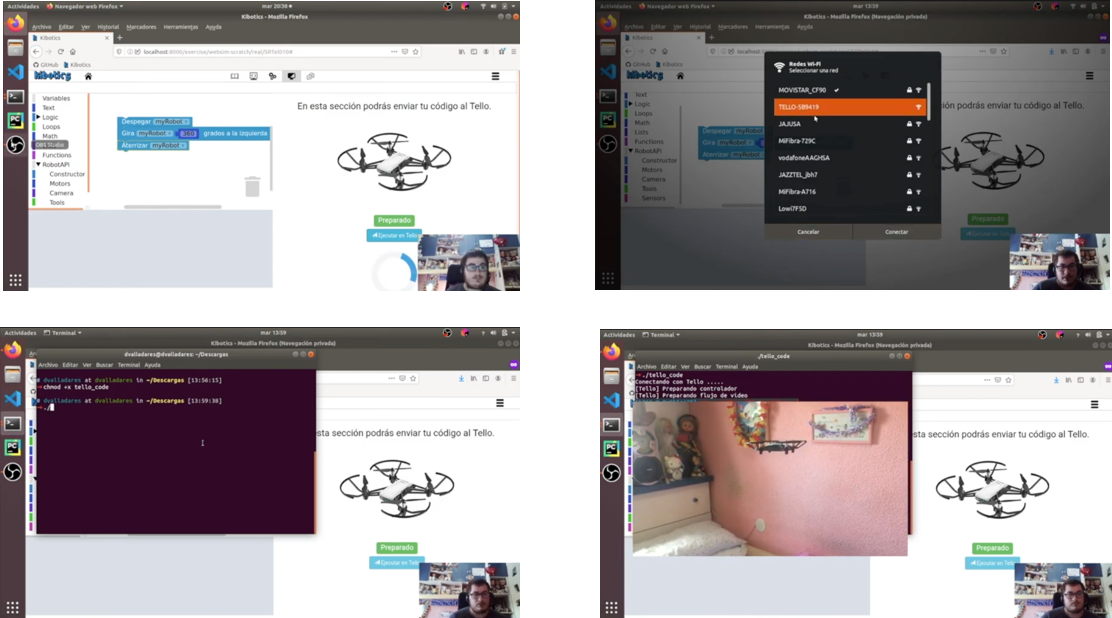
\includegraphics[width=1\textwidth]{images/fotogramas_tello.png}
  \caption{Fotogramas del vídeo de ejemplo de realización de un programa para el Tello en Linux}
  \label{Fotogramas del vídeo de ejemplo de realización de un programa para el Tello en Linux}
\end{figure}


%###############################################################################
%###################### GoPiGo ##################################################
%###############################################################################

\chapter{Integración del robot GoPiGo3}

Al igual que en los capítulos anteriores, mostraremos cuál ha sido el desarrollo realizado para llevar, en este caso, el robot GopiGo3 a la plataforma Kibotics, lo que permitirá su programación.

\section{Características del Robot GoPiGo3}

GoPiGo es un robot fabricado por Dexter Industries \footnote{\url{https://www.dexterindustries.com}}, que pretende integrar la Raspberry Pi en los robots, dotándoles así de una mayor capacidad y flexibilidad. Actualmente se encuentra en su versión GoPiGo3, que consiste en un kit robótico con forma de vehículo (Figura 6.1).
\\
\begin{figure}[h!]
  \centering
    \includegraphics[width=0.8\textwidth]{images/partes_GoPiGo.png}
  \caption{Diseño hardware del GopiGo3}
  \label{Diseño hardware del GopiGo3}
\end{figure}
\\
Entre las características del \textit{hardware} del GoPiGo3 destaca su cuerpo, que consiste en un acrílico grueso. Requiere un voltaje de entre 7-12V, conseguible con una batería a pilas. Dispone de una placa llamada “GoPiGo3", que se conecta a la Raspberry Pi. La comunicación con la controladora se produce a través de la interfaz SPI (\textit{Serial Peripheral Interface}). Incluye dos motores para conectarlo a las ruedas, las cuales tienen 66,5 mm de diámetro. También dispone de codificadores electrónicos, que se conectan a los motores para mejorar la movilidad. Respecto a las interfaces externas, destacan los dos puertos I2C (\textit{Inter-Integrated Circuit}) y los puertos serie que están acoplados a los pines de la Raspberry Pi (Dexter Industries, 2020).
\\
\\
Dexter Industries también ha desarrollado DexterOS, que incluye el \textit{software} necesario para que la Raspberry Pi funcione con GoPiGo3 (Dexter Industries, 2020). DexterOS se distribuye mediante una SD (\textit{Secure Digital}) de 8GB que se inserta en la ranura de la Raspberry Pi. Este \textit{software} emite una señal \textit{WiFi} que, una vez que el usuario se ha conectado a ese punto de acceso, al acceder al navegador se obtiene una web que permite interactuar con el robot sin necesidad de realizar ninguna descarga previa en el ordenador (Figura 6.2).
\\
\begin{figure}[h!]
  \centering
    \includegraphics[width=0.6\textwidth]{images/software_GoPiGo.png}
  \caption{Sotfware para GoPiGo3}
  \label{Sotfware para GoPiGo3}
\end{figure}
\\
Esta web dispone de cuatro módulos. El primero incluye lecciones integradas para aprender a programar el GoPiGo3 y algunos conceptos sobre los sensores de los que dispone. Otro módulo ofrece la posibilidad de conducir el GoPiGo3 de forma remota. Los otros dos módulos sirven como editores para programar el robot, de manera que uno de ellos permite programarlo mediante un lenguaje basado en bloques llamado \texttt{Bloxter} (Figura 6.3), muy similar a \texttt{Blockly} y diseñado por la propia empresa, mientras que el otro sirve para programarlo en \texttt{Python} (Dexter Industries, 2020). También han creado librerías que facilitan su programación para este lenguaje (una de ellas se llama \texttt{EasyGoPiGo3}).
\\
\begin{figure}[h!]
  \centering
    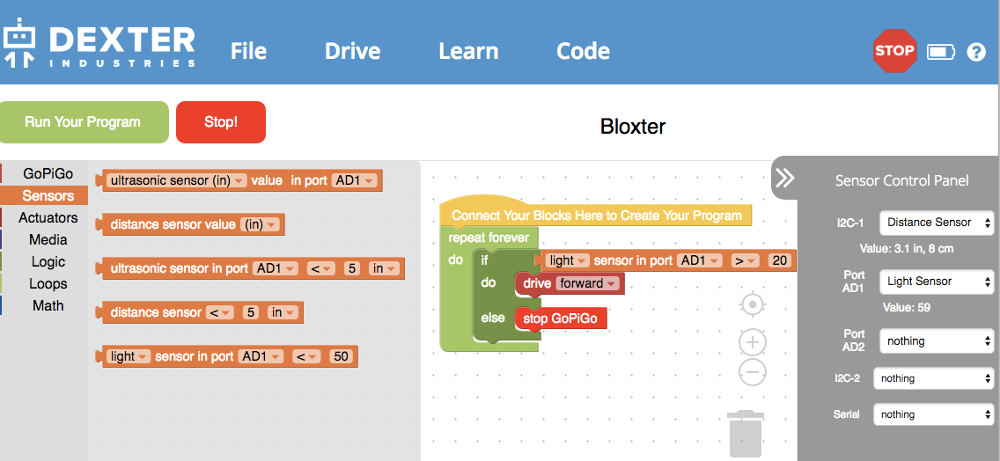
\includegraphics[width=0.6\textwidth]{images/editor_bloxter.png}
  \caption{Editor para el lenguaje Bloxter}
  \label{Editor para el lenguaje Bloxter}
\end{figure}

\section{Diseño}

La figura 6.4 muestra el diseño seguido para integrar el GoPiGo3 real a la plataforma Kibotics. En comparación con el diseño para los dos robots anteriores, en este caso se utiliza un servidor adicional \texttt{Flask} que permitirá la recepción del programa en el robot en su procesador Raspberry Pi.
\\
\begin{figure}[h!]
  \centering
    \includegraphics[width=0.8\textwidth]{images/arquitectura_GoPiGo.png}
  \caption{Diseño para la integración del GoPiGo3. La línea roja indica los componentes que deben estar conectados a la misma red WiFi}
  \label{Diseño para la integración del GoPiGo3}
\end{figure}
\\
El proceso consta de 5 pasos y en las siguientes secciones se profundizará en cada una de las partes y en las interacciones necesarias entre el cliente, el servidor de Kibotics y el servidor \texttt{Flask} de la Raspberry Pi, que permitirá programar al GoPiGo3 desde el navegador web usando Kibotics.

\section{Lado Cliente}

En la parrilla de unidades de Kibotics, se pueden encontrar varios ejercicios dedicados al GoPiGo3 para \texttt{Python}. Actualmente solo está disponible para este lenguaje.
\\
\\
En una de secciones del ejercicio se proporciona información al usuario sobre cómo realizar el envío, así como de las instalaciones que deben realizar. En este caso solo tiene que hacer instalaciones en la Raspberry Pi del robot, ya que en el ordenador del anfitrión no es necesaria ninguna instalación. En el fragmento 6.1 se muestran los detalles de cómo se ha diseñado esta sección.
\\
\begin{lstlisting}[frame=single,breaklines=true, label=Página de información del GoPiGo3, caption=Página de información del GoPiGo3,  captionpos=b]
<html>
<head>
<meta charset='UTF-8'><meta name='viewport' content='width=device-width initial-scale=1'>
<title>GoPiGo3</title></head>
<body><h1>GoPiGo3 example</h1>
<p>Podras realizar tu programa para enviarselo al GoPiGo.</p>
<p><img src="" width=200px></p>

<h2>1 - Instalacion</h2>
<ul>
 <li type="circle">
  <h4>   <b>En la Raspberry Pi 3 del GoPiGo3:</b> </h4>
   <ol start='1' >
    <li>
     Descargar el siguiente fichero comprimido => <a href="" target="_blank">Intalador</a>
    </li>
    <li>
     Descomprimir el Zip descargado y situarlo en el directorio /home/pi/
    </li>
    <li>
     Ir al directorio e instalar los drivers necesario, para ello abrir un terminal y ejecutar
    </li>
    <ol start='1' >
     <li>
      <code>chmod +x instalar_drivers_GoPiGo.sh</code>
     </li>
     <li>
      <code>./instalar_drivers_GoPiGo.sh</code>
     </li>
    </ol>
    <li>
     Agregar la instruccion que permite levantar siempre el servidor al encenderse la Raspberry, para ello dirigirse al directorio y abrir un terminal:</li> 
     <ol start='1' >
      <li>
       Ejecutar => <code>chmod +x iniciar_servidor_GoPiGo.sh</code>
      </li> 
      <li>
       Abrir el servicio cron => <code>crontabl -e</code>
      </li> 
      <li>
       Agregar la tarea <code> @reboot /home/pi/configuracion_GoPiGo/iniciar_servidor_GoPiGo.sh &</code>
      </li> 
     </ol>
   </ol>
   </li>
   <li type="circle">
    <h4>   <b>En el ordenador MacOS/Linux/Windows:</b> </h4>
     <p>No es necesaria ningun tipo de instalacion adicional para el funcionamiento.</p>
    </li>
</ul>

<h2>2 - Ejecucion</h2>
<ol start='' >
 <li>
  Realice su programa
 </li>
  <li>
   Eciende el GoPiGo y asegurate de que esta conectado a el WiFi. 
  </li>
  <li>
   Pulse en <b>Enviar</b>, si todo ha ido bien se cargara el programa en el GoPiGo3. 
  </li>
</ol>
</body>
</html>
\end{lstlisting}

\subsection{Editor en el navegador web}

Para escribir un programa y enviarlo al robot desde el lado del cliente, otra sección de la página web del ejercicio proporciona un editor donde el usuario podrá escribir su programa utilizando el lenguaje \texttt{Python}. En el editor se importa la librería “\texttt{EasyGoPigo3}” (Dexter Industries, 2018), que proporciona una API para interactuar con los sensores y actuadores del robot (Figura 6.5).
\\
\begin{figure}[h!]
  \centering
    \includegraphics[width=1\textwidth]{images/editor_gopigo3.png}
  \caption{Editor python para el GoPiGo3}
  \label{Editor python para el GoPiGo3}
\end{figure}
\\

\subsection{Envío del código al servidor Flask en el robot}

Una vez que el usuario ha escrito el programa deseado, deberá pulsar el botón “Enviar” que puede verse en la figura 6.5, el cual desencadenará todo el proceso de envío. En el fragmento 6.2 se muestra cuál es el código HTML que permite iniciar este proceso.
\\
\begin{lstlisting}[frame=single,breaklines=true, label=Sección para el envío, caption=Sección para el envío,  captionpos=b]
<center><h3>En esta seccion podras enviar tu codigo  al GoPiGo3.</h3></center>

<div class="text-center">
 <img class="text-center" src="{{ exercise.language }}/{{ exercise.exercise_id }}/img/GoPiGo3.png" width="300px" height="250px">
</div>

<div id="text" class="text-center">
 <h3><span id="proxy_state" class="label label-success">Conexion con proxy</span></h3>
  <button type="button" id="send_mbot" class="btn btn-info" onclick="send_code_to_GoPiGo()">
   <span class="glyphicon glyphicon-send"></span> Enviar
  </button>
</div>
\end{lstlisting}
Tras pulsar el botón de envío, desde el navegador se manda al servidor \texttt{Flask} levantado en la Raspberry Pi del robot, el código del programa que se había escrito previamente en el editor. Este código se envía como un \textit{query parameter} de una petición GET haciendo uso de la función \texttt{fecth()}, de forma similar que en los capítulos anteriores.
\\
\begin{lstlisting}[frame=single,breaklines=true, label=Función de envío del código al servidor del GopiGo3, caption=Función de envío del código al servidor del GopiGo3,  captionpos=b]
function send_code_to_GoPiGo() {
   var editor = ace.edit("ace");
   let code = editor.getValue();
   console.log(code);
   const message = {
      method: "GET"
   };
   url = 'http://192.168.1.200:8001/run?python_code=' + JSON.stringify(code);
   fetch(url, message)
      .then(function(response) {
         if(response.ok){
            responseOk = true
         }else{
            responseOk = false
         }
           return response.text();
         })
      .then(function(data) {
         if(responseOk){
            console.log("Ok")
         }else{
            console.log("Send Fail")
         }

      })
      .catch(function(err) {
         console.error(err);
      });
}
\end{lstlisting}
El servidor \texttt{Flask} recibirá el código y realizará una serie de acciones (sección 6.5) que permitirán cargar el programa al robot.

\section{Lado Servidor Kibotics}

Este servidor no toma un papel tan importante para el proceso de envío del programa al GoPiGo3 como sí lo tenía para el Mbot y el dron Tello. En ellos, además de servir las páginas necesarias al navegador que permiten ir al ejercicio concreto del robot, a la sección de información o al editor, era el encargado de manipular el código fuente, de crear el ejecutable o de realizar el empaquetado que se enviaba al robot.
\\
\\
En este diseño, una vez que el código está escrito en el editor web, es enviado al servidor de kibotics para el guardado del ejercicio del usuario y al servidor \texttt{Flask} del robot para procesarlo y ejecutarlo. 

\section{Lado GoPiGo3}

La Raspberry Pi del GoPiGo3 toma un papel muy importante en el proceso de envío del programa al robot, puesto que en ella se tendrá montado un servidor \texttt{Flask} HTTP, que recibirá las peticiones del cliente y contendrá la lógica para la ejecución del programa recibido.
\\
\\
A diferencia del ordenador anfitrión, donde no se requería ninguna instalación para el envío del programa, en la Raspberry Pi sí hay que realizar unas instalaciones previas para poder utilizarse en el GopiGo3.

\subsection{Preparación del ordenador a bordo del GoPiGo3}

La preparación de la Raspberry Pi requiere una serie de procesos.

\begin{enumerate}
	\item \textit{Instalar sistema operativo}
	\\
	\\
	La Raspberry Pi necesita un sistema operativo. Aunque existen varios que puede soportar, se debe utilizar \texttt{Raspbian}, un sistema operativo optimizado para ella y basado en Debian, una distribución GNU/Linux.
	\item \textit{Instalación de los drivers y configuración} 
	\\
	\\
	Se deben instalar los \textit{drivers} y las librerías necesarias para que pueda interactuar con los sensores y actuadores del robot GoPiGo3. También es indispensable que esté conectada a la misma red \textit{WiFi} que el ordenador anfitrión, así como tener asignada la IP (Protocolo de Internet) fija \texttt{192.168.1.200}. Si esto no se cumple, cada vez que se encienda la Raspberry Pi, tendrá una IP distinta y no podrá realizarse el envío.
	\\
	\\
	En la página de información del ejercicio para el GoPiGo3 en Kibotics se le proporciona al usuario un fichero comprimido que contiene un ejecutable que instalará los \textit{drivers} y configurará la IP fija, evitando así que sea el usuario quien tenga que hacerlo (Fragmento 6.4).
	\\
	\begin{lstlisting}[frame=single,breaklines=true, label=Ejecutable para la instalación y configuración de la Raspberry Pi, caption=Ejecutable para la instalación y configuración de la Raspberry Pi,  captionpos=b]
#!/bin/bash

######### Instalacion GoPiGo3 #############

echo "Instalando GoPiGo3"
curl -kL dexterindustries.com/update_GoPiGo3 | bash

echo "Intalacion GoPiGo3 completa"

######## Actualizar el firmware GoPiGo3 ####

echo "Actualizando firmware de GoPiGo3"

mv ~/Dexter/GoPiGo3/Firmware/archives/GoPiGo3_Firmware_0.3.4.bin ~/Dexter/GoPiGo3/Firmware/
rm ~/Dexter/GoPiGo3/Firmware/GoPiGo3_Firmware_1.0.0.bin
chmod +x ~/Dexter/GoPiGo3/Firmware/GoPiGo3_flash_firmware.sh
bash ~/Dexter/GoPiGo3/Firmware/GoPiGo3_flash_firmware.sh

echo "Finalizada actualizacion firmware para GoPiGo3"

###### Crear entorno virtual ###

echo "Creando entorno virtual python3"

python3 -m venv ~/.virtualenvs/GoPiGo
source ~/.virtualenvs/GoPiGo/bin/activate
pip install GoPiGo3
pip install numpy
pip install pandas
pip install Flask
deactivate

echo "Finalizado Creacion de entonro virtual"

### Configurar ip estatica ###

echo "Configurando ip estatica"

sudo service dhcpcd status
sudo service dhcpcd start
sudo systemctl enable dhcpcd

echo -e "\ninterface wlan0\nstatic ip_address=192.168.1.200/24\nstatic routers=192.168.1.1\nstatic domain_name_servers=192.168.1.1" >> /etc/dhcpcd.conf

echo "Configurada ip estatica"

echo "##########################"
echo "### Proceso Completado ###"
echo "##########################"

read -p "Necesitas reiniciar. Quieres tu reiniciarl la maquina? [y/n]: " restart
if [ "$restart" = "y" ]; then
        sudo reboot
fi
	\end{lstlisting}
	\item \textit{Montaje del servidor Flask}
	\\
	\\
	El fichero comprimido también contiene el código fuente que permite crear el servidor HTTP. El servidor se ha desarrollado con el lenguaje \texttt {Python} y haciendo uso de \texttt{Flask}, un entorno escrito en \texttt{Python} que permite crear servidores webs.
	\\
	\\
	Es necesario que este servidor se lance una vez que se encienda la Raspberry Pi de manera automática, ya que si no, es el usuario quien tendría que lanzarlo cada vez que se encienda. Para ello hacemos uso del servicio \texttt{cron}, un administrador de tareas en \texttt{Linux} que permite programar el lanzamiento de comandos en un determinado momento (Dinahosting, s.f.).
	\\
	\\
	Para programar el lanzamiento del servidor de manera automática al encenderse el robot, el usuario deber realizar las siguientes acciones:
	\begin{enumerate}
		\item Descomprimir el fichero descargado en el directorio \textit{/home/pi/} y dar permiso de ejecución al ejecutable \textit{iniciar\_servidor\_GoPiGo.sh}
		\item Abrir un terminal y ejecutar:  \textit{crontab -e}
		\item Añadir la tarea: \textit{@reboot /home/pi/configuración\_GoPiGo/iniciar\_servidor\_GoPiGo.sh}
		\item Reiniciar el servicio cron: \textit{sudo /etc/init.d/cron restart}
	\end{enumerate}
\end{enumerate}

\subsection{Recepción a bordo del código fuente}

El servidor \texttt{Flask} del GoPiGo3 recibe la petición del navegador con el código extraído del editor, donde el usuario escribió el programa.
\\
\begin{lstlisting}[frame=single,breaklines=true, label=Extracción del código en el servidor del GoPiGo3, caption=Extracción del código en el servidor del GoPiGo3,  captionpos=b]
exercice = None
@app.route('/run',methods=["GET"])
def run_program():
   global exercice
   code = request.args.get('python_code')
    . . .
\end{lstlisting}

\subsection{Creación del proceso que ejecuta la aplicación robótica}

El robot GoPiGo3 entiende el lenguaje \texttt{Python} porque tiene un intérprete de \texttt{Python} ya instalado, de manera que una vez extraído el código del usuario, no es necesario realizar ningún tipo de conversión.
\\
\\
Se tiene que crear un proceso que ejecute el código recibido. Para ello es necesario crear un ejecutable \texttt{Python} (extensión .py) y empotrarle el código extraído. Podría ocurrir que el robot ya estuviera ejecutando un programa, por lo que antes de lanzar el nuevo programa, se tiene que verificar si ya se está ejecutando otro en él y, en tal caso, “matar” al proceso que lo ejecuta.
\\
\\
Tras ejecutar el programa en un nuevo proceso, el robot realizará las instrucciones que el usuario programo en el editor del navegador web.
\\
\begin{lstlisting}[frame=single,breaklines=true, label=Creación del proceso con el programa para el robot, caption=Creación del proceso con el programa para el robot,  captionpos=b]
# Stop process have alreay up
if exercice:
   try:
      os.killpg(os.getpgid(exercice.pid), signal.SIGKILL)
   except ProcessLookupError:
      pass

time.sleep(2)
    
# Creat exercice.py
code  = code[1:-1].split("\\n")
fdOut = open("./ejercicio.py","w")
for line in code:
   fdOut.write(line + "\n")
    
# Run process
exercice = subprocess.Popen(["python","ejercicio.py"],stdout=subprocess.PIPE,preexec_fn=os.setsid)
\end{lstlisting}

\section{Validación experimental}

Una vez mostrado el diseño que permite programar el GoPiGo3 desde la plataforma Kibotics, podemos observar la flexibilidad y operatividad que tiene este robot gracias a la Raspberry Pi que lleva integrada.
\\
\\
Una de las ventajas que ofrece este diseño es que el proceso de envío es independiente del sistema operativo que utiliza el usuario. Esto es posible porque el programa se escribe en el navegador y se envía directamente al servidor \texttt{Flask} montado en el robot, consiguiendo así que el diseño, además de ser multiplataforma, sea “cero-instalación” para el ordenador del anfitrión.
\\
\\
En cuanto al robot, al ser necesaria una preparación previa, puede ser algo más complejo para los usuarios de menor edad o que acaban de iniciarse en la informática. Por ello, se proporcionan ejecutables (mencionados en la sección 6.5.1), encargados de la instalación e instrucciones para minimizar y facilitar este proceso.
\\
\\
Por otro lado, la integración del GoPiGo3 ha sido probada tanto para diferentes sistemas operativos (\texttt{Ubuntu 18.04}, \texttt{Ubuntu 16.04}, \textit{Windows 10}, \texttt{Windows 7}, \texttt{MacOS Catalina Versión 10.15.6}, \texttt{MacOS Mojave Versión 10.14.6}), así como en diferentes navegadores (\texttt{Safari Versión 14.0}, \texttt{Google Chrome Versión 85.0}, \texttt{Firefox Versión 68.9}).
\\
\\
En los siguientes punteros a videos se puede visualizar un ejemplo de realización de un programa y envío al GoPiGo3 desde la plataforma Kibotics:
\begin{itemize}
	\item \textbf{\texttt{MacOS}:} \textit{\url{https://youtu.be/ziuRS14VhIM}}
	\item \textbf{\texttt{Windows}:}  \textit{\url{https://youtu.be/R7S6J35FT\_A}}
	\item \textbf{\texttt{Linux}:}  \textit{\url{https://youtu.be/l5Qtx3Ne8Cw}}
\end{itemize}
En la figura 6.6 se muestran varios fotogramas del vídeo de ejemplo para el proceso de envío de un programa al GoPiGo3 en \texttt{MacOS}. El primer  paso es realizar el programa deseado. Posteriormente, al pulsar en el botón de enviar, el programa se ejecuta en el robot. Este proceso seria similar para \texttt{Linux} y \texttt{Windows}.
\begin{figure}[h!]
  \centering
    \includegraphics[width=1\textwidth]{images/fotograma_ejercicio_GoPiGo.png}
  \caption{Fotogramas del vídeo de ejemplo de realización de un programa para el GoPiGo3 en MacOS}
  \label{Fotogramas del vídeo de ejemplo de realización de un programa para el GoPiGo3 en MacOS}
\end{figure}

%###############################################################################
%###################### Conclusiones #############################################
%###############################################################################

\chapter{Conclusiones}

Tras explicar los objetivos, herramientas, etapas y procesos necesarios para llevar a cabo el desarrollo de este TFG, finalmente en este capítulo se especificarán las conclusiones principales y las posibles líneas de investigación futuras derivadas de este proyecto.

\subsection{Conclusiones}

Una vez que se ha analizado el trabajo realizado, se puede afirmar que sí se cumple el objetivo principal planteado, pues hemos conseguido llevar los robots Mbot, Tello y GopiGo3 a la plataforma Kibotics y programarlos desde ella.
\\
\\
Por otro lado, también podríamos decir que se cumple el primer objetivo específico mencionado en el capítulo 2, ya que se ha conseguido que las integraciones de los robots sean multiplataforma, de manera que ahora todos ellos se pueden programar con \texttt{Linux}, \texttt{Windows} y \texttt{MacOS}. Respecto al segundo subobjetivo, sí se ha conseguido facilitar el proceso de envío en todos los casos, aunque por las propias características de los robots, en algunos casos se necesitan instalaciones previas:
\begin{itemize}
	\item En el Mbot, gracias a la tecnología \texttt{Web Serial} se ha conseguido que el usuario no necesite hacer ninguna instalación ni configuración previa para utilizar el robot. Además, el envío se ha simplificado mucho, pues el ejercicio se envía directamente al robot una vez que el usuario lo haya realizado. Este proceso es similar en los tres sistemas operativos.
	\item En el dron Tello, el proceso de envío no es tan directo como en el caso anterior, lo que se debe, en gran parte, a que no se tiene ningún tipo de control sobre la controladora del robot y a que para comunicarse con el dron hay que estar conectado al \textit{WiFi} que emite. Por otra parte, también hay diferencias entre los sistemas operativos; en \texttt{Linux} sí se ha conseguido que el usuario no tenga que hacer ninguna instalación en el ordenador, y el envío del programa se limita a lanzar un ejecutable que comunicará con el Tello. En el caso de \texttt{Windows} y \texttt{MacOS} se necesita que el usuario tenga instalado unos requisitos en su ordenador, pero en el caso de \texttt{MacOS} se ha diseñado un ejecutable que le facilita todas las instalaciones y configuraciones necesarias.
	\item En el GopiGo3 se necesita una preparación previa en el robot, pero esto se debe a que al llevar integrada una Raspberry Pi hay que instalar los \textit{drivers} para configurarla con el robot y preparar el servidor alojado en él. Esto permite comunicarnos desde otros dispositivos con él. Para facilitar esta preparación, se le ha proporcionado al usuario unos ejecutables que instalarán y configurarán todo lo necesario. En el caso del ordenador del usuario, no se necesita una instalación previa y el proceso de envío es directo para cualquiera de los sistemas operativos gracias al servidor montado en el robot.
\end{itemize}
Por otro lado, el proceso de elaboración de este TFG ha permitido estudiar en profundidad diferentes ámbitos de la robótica y de la informática gracias al manejo de los tres robots y a la necesidad de que sean multiplataforma. Entre las nuevas competencias adquiridas, destacan los siguientes puntos:
\begin{itemize}
	\item Introducción en la Robótica Educativa y aspectos del \textit{hardware} y \textit{software} de los robots utilizados.
	\item Profundizar en el manejo de lenguajes de programación (\texttt{Python}, \texttt{JavaScript}, \texttt{Shell}).
	\item Adquirir conocimientos en desarrollo web utilizando \texttt{HTML}, Bootstrap, Django y Flask.
	\item Mejorar la formación sobre los sistemas operativos \texttt{Linux}, \texttt{Windows}, \texttt{MacOS} y \texttt{Raspbian}.
	\item Aprender el manejo de una \texttt{Raspberry Pi}.
	\item Estudiar las tecnologías \texttt{Web Serial}, \texttt{PyInstaller}.
	\item Mejorar la habilidad sobre el desarrollo de software, así como \texttt{Git} y \texttt{GitLab}.
	\item Aprender el manejo de Latex, la aplicación utilizada para la redacción de este TFG
\end{itemize}

\subsection{Líneas futuras}

Con la realización de este TFG surgen una serie de líneas de investigación futuras que pueden resultar útiles para seguir mejorando la plataforma de Kibotics.
\\
\\
En primer lugar, la tecnología \texttt{Web Serial} abre un camino bastante interesante al permitir una comunicación con dispositivos conectados al puerto serie vía web. Con ella puede utilizarse para comunicarse directamente desde el navegador, consiguiendo así que sea multiplataforma. Existen muchos dispositivos que necesitan una conexión USB, por lo que esta opción sería una buena forma de comunicación con ellos.
\\
\\
Por otro lado, en el caso del GopiGo3, el hecho de tener un ordenador instalado va a permitir realizar muchas acciones en este robot. Actualmente solo está disponible en \texttt{Python}, por lo que una línea de investigación podría centrarse en adaptar su uso al lenguaje \texttt{Blockly} para que puedan utilizarlo niños de menor edad. Además, la potencia que presenta este robot posibilita el diseño de ejercicios muy interesantes, por ejemplo, si le instalamos una cámara, el robot sería capaz de realizar ejercicios de visión artificial.




%###############################################################################
%###################### Biografia #################################################
%###############################################################################

\chapter{Bibliografía}

Báez, M.; Bongiovanni, P.; Castrillejo, D.; García, J. M.; Leal, D.; Levis, D.; Lugo, M. T.; Maguregui, C.; Ochoa, G.;  Peña-López, I.; Pisano, R.; Rabajoli, G.; Rivoir, A.; Sansberro, F.; Turner, N.; Vacca, A. M.; Vaillant, D. (2011).  \textit{El modelo CEIBAL. Nuevas tendencias para el aprendizaje}. Uruguay: CEIBAL - ANEP.
\\
\\
Bravo, F. Á.; Forero, A. (2012). \textit{La robótica como un recurso para facilitar el aprendizaje y desarrollo de competencias generales}. Teoría de la Educación. Educación y Cultura en la Sociedad de la Información 13(2): 120-139.
\\
\\
Castro, G. (6 de junio de 2019).  \textit{DJI Tello, un minidron de juguete, programable con un procesador potentísimo}. DronProfesional. Recuperado de https://dronprofesional.com/blog/dji-tello-un-minidron-de-juguete-programable-con-un-procesador-potentisimo/
\\
\\
Challenger, I.; Díaz, Y.; Becerra, R. A. (2014). \textit{El lenguaje de programación Python}. Ciencias Holguín, 20(2): 1-13
\\
\\
Cumplido, A. (16 de febrero de 2018).  \textit{El origen de Bootstrap, el framework CSS líder}. Webtraining Blog. Recuperado de https://blog.webtraining.zone/el-origen-de-bootstrap-el-framework-css-lider/
\\
\\
Curso de iniciación a Python en Raspberry Pi. (2020). Recuperado 12 de septiembre de 2020, de Asociación Programo Ergo Sum website: https://www.programoergosum.com/cursos-online/raspberry-pi/244-iniciacion-a-python-en-raspberry-pi/que-es-python
\\
\\
Dexter Industries (2020). \textit{GopiGo3 is a RaspberryPi Robot Car for Learning Coding}. Recuperado el 27 de septiembre de 2020 de https://www.dexterindustries.com/gopigo3/
\\
\\
Dexter  Industries (2018). 5.1.  \textit{About library and Hardware}. https://gopigo3.readthedocs.io/en/master/api\-basic/structure.html
\\
\\
Dinahosting (s.f.). \textit{¿Qué es cron y para qué sirve? - Ayuda de dinahosting}. https://dinahosting.com/ayuda/como-configurar-tareas-cron-de-forma-manual/
\\
\\
Eguíluz, J. (2009). Introducción a JavaScript. Recuperado de https://uniwebsidad.com/libros/javascript
\\
\\
Escuela Técnica Superior de Ingeniería Informática de la Universidad Politécnica de Valencia (18 de diciembre de 2013). Raspberry Pi.  \textit{Historia de la Informática}. Recuperado de https://histinf.blogs.upv.es/2013/12/18/raspberry-pi/
\\
\\
González, J. J.; Jiménez, J. A. (2009). \textit{La robótica como herramienta para la educación en ciencias e ingeniería}. \textit{IE Comunicaciones: Revista Iberoamericana de Informática Educativa} 10: 31-36.
\\
\\
Guevara, A. (s.f.). \textit{¿Qué es Bootstrap?}. Devcode. Recuperado de https://devcode.la/blog/que-es-bootstrap/
\\
\\
Holovaty, A.; Kaplan-Moss, J. (2007).  \textit{El libro de Django}. Recuperado de http://bibing.us.es/proyectos/abreproy/12051/fichero/libros\%252Flibro-django.pdf
\\
\\
Lamarca, M. J. (2018). \textit{Hipertexto, el nuevo concepto de documento en la cultura de la imagen}. http://www.hipertexto.info/documentos/html.htm
\\
\\
Novapros (21 de abril de 2020). \textit{¿Qué es Django framework y quienes lo usan?}. Novapros Blog. Recuperado de https://novapros.es/blog/que-es-django-framework-y-quienes-lo-usan/
\\
\\
Moreno, I.; Muñoz, L.; Serracín, J. R.; Quintero, J.; Patiño, K. P.; Quiel, J. (2012).\textit{ La robótica educativa, una herramienta para la enseñanza-aprendizaje de las ciencias y las tecnologías. Teoría de la Educación. Educación y Cultura en la Sociedad de la Información} 13(2): 74-90.
\\
\\
PYPL PopularitY of Programming Language index. (2020). Recuperado 15 de septiembre de 2020, de PYPL PopularitY of Programming Language website: http://pypl.github.io/PYPL.html
\\
\\
Quiroga, L. P. (2018). \textit{La robótica: otra forma de aprender. Revista Educación y Pensamiento} 25(25): 51-64
\\
\\
Raggett, D.; Le Hors, A.; Jacobs, I. (1999). HTML 4.01 Specification. W3C recommendation, 24.
\\
\\
Robótica Educativa con Mbot. (2020). Recuperado 19 de septiembre de 2020, de Programo Ergo Sum website: https://www.programoergosum.com/cursos-online/robotica-educativa/249-robotica-educativa-con-mbot/que-es-mbot
\\
\\
Rodríguez, X. (21 de agosto de 2019).  \textit{Django vs Flask. Openwebinars}. Recuperado de https://openwebinars.net/blog/django-vs-flask/
\\
\\
REAL ACADEMIA ESPAÑOLA: \textit{Diccionario de la lengua española}, 23.ª ed., [versión 23.3 en línea]. <https://dle.rae.es> [12 de septiembre de 2020].
\\
\\
Ruiz-Velasco, E.; García, J. V.; Rosas, L. A. (2007). \textit{Robótica pedagógica virtual para la inteligencia colectiva}. México: Universidad Nacional Autónoma de México.
\\
\\
Salamanca, M. L.; Barrera, N.; Pérez, W. J. (2010). \textit{Uso de la robótica educativa como herramienta en los procesos de enseñanza}. Ingeniería Investigación y Desarrollo: I2+D 10(1): 15-23.
\\
\\
Shannon, R. E. (1998, diciembre 13-16). \textit{Introduction to the art and science of simulation}. In 1998 Winter Simulation Conference. Doi: 10.1109/WSC.1998.744890
\\
\\
SO Documentation (s.f.).  \textit{PyInstaller - Distribuir código de Python}.  https://sodocumentation.net/es/python/topic/2289/pyinstaller---distribuir-codigo-de-python
\\
\\
Valladares, D. (18 de diciembre de 2019). My blog. My TFG’s blog. Recuperado de https://roboticslaburjc.github.io/2019-tfg-david-valladares/
\\
\\
Valladares, D. [David Valladares vigara]. (2020, Septiembre, 5). \textit{Gopigo3 by WiFi} [Archivo de vídeo]. Recuperado de https://youtu.be/jHZ\_GBfIB5I
\\
\\
Valladares, D. [David Valladares vigara]. (2020, Septiembre, ). \textit{Gopigo3 by WiFi} [Archivo de vídeo]. Recuperado de
\\
\\
Valladares, D. [David Valladares vigara]. (2020, Septiembre, ). \textit{Gopigo3 by WiFi} [Archivo de vídeo]. Recuperado de
\\
\\
W3C Community Group (2020). \textit{Serial Api Living document}. https://wicg.github.io/serial/
\\
\\
Zaforas, M. (2018). \textit{¿Es Python el lenguaje del futuro?}. Paradigma Digital. Recuperado de https://www.paradigmadigital.com/dev/es-python-el-lenguaje-del-futuro/
\end{document}
